\documentclass[11pt,a4paper]{article}
\usepackage[spanish,es-nodecimaldot,es-noshorthands]{babel}
\usepackage[utf8]{inputenc}
\usepackage[margin=2.2cm, top=3.2cm, headheight=2.2cm]{geometry}
\usepackage{graphicx}
\usepackage{booktabs}
\usepackage{tabularx}
\usepackage{xcolor}
\usepackage{amsmath,amssymb}
\usepackage{listings}
\usepackage{xurl}
\usepackage{hyperref}
\usepackage{fancyhdr}
\usepackage{caption}
\usepackage{subcaption}
\usepackage{float}
\usepackage{enumitem}
\usepackage{array}

\definecolor{utared}{RGB}{180, 20, 20}
\definecolor{utagray}{RGB}{247, 248, 250}
\definecolor{navyblue}{RGB}{0, 51, 102}

\hypersetup{
    colorlinks=true,
    linkcolor=navyblue,
    citecolor=navyblue,
    urlcolor=navyblue,
    breaklinks=true
}

\lstset{
    language=Python,
    basicstyle=\ttfamily\footnotesize,
    keywordstyle=\color{blue}\bfseries,
    stringstyle=\color{teal},
    commentstyle=\color{gray}\itshape,
    backgroundcolor=\color{utagray},
    frame=single,
    rulecolor=\color{lightgray},
    breaklines=true,
    showstringspaces=false,
    tabsize=4
}

% Encabezado y Pie de Página Institucional
\pagestyle{fancy}
\fancyhf{}
\fancyhead[L]{
\includegraphics[height=1.4cm]{images/logo_uta.png}}
\fancyhead[C]{%
    \textbf{\fontsize{11}{13}\selectfont UNIVERSIDAD TÉCNICA DE AMBATO}\\[2pt]
    \textbf{\fontsize{9}{11}\selectfont FACULTAD DE INGENIERÍA EN SISTEMAS ELECTRÓNICA E INDUSTRIAL}\\[2pt]
    \textbf{\fontsize{8.5}{10.5}\selectfont CARRERA DE INGENIERÍA EN SOFTWARE / COMPUTACIÓN}\\[2pt]
    \textbf{\fontsize{8}{10}\selectfont CICLO ACADÉMICO: JULIO -- DICIEMBRE 2026}
}
\fancyhead[R]{
\includegraphics[height=1.4cm]{images/logo_fisei.png}}
\fancyfoot[C]{\thepage}
\renewcommand{\headrulewidth}{1.2pt}
\renewcommand{\footrulewidth}{0.5pt}

\begin{document}

\begin{center}
    {\Large \textbf{INFORME DE GUÍA PRÁCTICA}}\\[0.3cm]
\end{center}

\section*{I. PORTADA}
\vspace{0.1cm}
\noindent
\begin{tabularx}{\textwidth}{@{}p{6.8cm}X@{}}
\textbf{Tema:} & Clasificación de dígitos manuscritos con MNIST \\[6pt]
\textbf{Unidad de Organización Curricular:} & Profesional \\[6pt]
\textbf{Nivel y Paralelo:} & Octavo / A \\[6pt]
\textbf{Alumnos participantes:} & Fiallos Yanza Jonathan Josue \\
                                & Guevara Panimboza Steven Marlon \\[6pt]
\textbf{Asignatura:} & Inteligencia Artificial \\[6pt]
\textbf{Docente:} & Rubén Nogales \\
\end{tabularx}

\vspace{0.4cm}

\section*{II. INFORME DE GUÍA PRÁCTICA}

\subsection*{2.1 Objetivos}
\textbf{General:}
\begin{itemize}[leftmargin=*,noitemsep]
    \item Comparar el desempeño de un árbol de decisión, Random Forest y k-NN al clasificar dígitos manuscritos de MNIST mediante un protocolo común de entrenamiento y prueba.
\end{itemize}

\textbf{Específicos:}
\begin{itemize}[leftmargin=*,noitemsep]
    \item Preparar las imágenes de MNIST y reproducir los conjuntos de entrenamiento y prueba.
    \item Ajustar y evaluar los tres clasificadores con los mismos datos y calcular su exactitud y error en cada conjunto.
    \item Justificar la elección de un modelo a partir de las métricas de prueba y del análisis de sus errores.
\end{itemize}

\subsection*{2.2 Modalidad}
Práctica en parejas, con ejecución en laboratorio y elaboración del informe fuera de clase.

\subsection*{2.3 Tiempo de duración}
\begin{itemize}[leftmargin=*,noitemsep]
    \item \textbf{Presenciales:} 2 horas para preparar los datos, entrenar y evaluar.
    \item \textbf{No presenciales:} 1 hora para comparar resultados y elaborar el informe.
\end{itemize}

\subsection*{2.4 Instrucciones}
Completen los datos de portada y registren los nombres en orden alfabético. Usen Python y conserven un solo cuaderno de trabajo por pareja. Mantengan la misma partición, transformación e hiperparámetros indicados para que los resultados puedan compararse.

Registren el entorno y las versiones de Python y scikit-learn. Completen las tablas con los resultados de su ejecución y numeren las figuras y tablas del informe.

\subsection*{2.5 Listado de equipos, materiales y recursos}
\begin{itemize}[leftmargin=*,noitemsep]
    \item Computador con conexión a Internet para la descarga inicial de MNIST \cite{openml_mnist}.
    \item Jupyter Notebook o Google Colab con Python, NumPy, pandas, scikit-learn y Matplotlib.
    \item \textbf{TAC:} Cuaderno interactivo para ejecutar código, visualizar imágenes y documentar los resultados.
\end{itemize}

\subsection*{2.6 Actividades por desarrollar}

\paragraph{Actividad 1. Preparar MNIST.}
Carguen \texttt{mnist\_784}, versión 1 (OpenML, ID 554) \cite{openml_mnist}. Cada imagen contiene $28 \times 28$ píxeles en escala de grises y tiene una etiqueta de 0 a 9. Visualicen cinco ejemplos con sus etiquetas.

Conserven la separación original: las primeras 60\,000 observaciones pertenecen a entrenamiento y las últimas 10\,000 a prueba. Para la práctica, tomen 10\,000 y 2\,000 observaciones, respectivamente, mediante muestreo estratificado por dígito con semilla 42. El Anexo A proporciona el código de partida.

Representen cada imagen como un vector de 784 intensidades entre 0 y 1, dividiendo por 255. Verifiquen las dimensiones de \texttt{X\_ent} y \texttt{X\_pru} y reporten cuántos ejemplos de cada dígito quedaron en ambos conjuntos.

\paragraph{Actividad 2. Entrenar.}
Instancien un objeto para cada modelo con la configuración de la Tabla~\ref{tab:configuracion}. Apliquen \texttt{fit(X\_ent, y\_ent)} a los tres, usando exactamente el mismo conjunto de entrenamiento.

\begin{table}[H]
\centering
\caption{Configuración de los clasificadores}
\label{tab:configuracion}
\renewcommand{\arraystretch}{1.2}
\begin{tabularx}{\textwidth}{l l X}
\toprule
\textbf{Modelo} & \textbf{Clase de scikit-learn} & \textbf{Hiperparámetros fijados} \\
\midrule
Árbol de decisión & \texttt{DecisionTreeClassifier} \cite{sklearn_dt} & \texttt{max\_depth=15, random\_state=42} \\
\addlinespace
Random Forest & \texttt{RandomForestClassifier} \cite{sklearn_rf} & \texttt{n\_estimators=100, max\_depth=15, random\_state=42} \\
\addlinespace
k-NN & \texttt{KNeighborsClassifier} \cite{sklearn_knn} & \texttt{n\_neighbors=5, metric="euclidean", weights="uniform"} \\
\bottomrule
\end{tabularx}
\end{table}

Usen los valores por defecto para los demás parámetros. Describan qué hace \texttt{fit} en cada modelo: el árbol aprende reglas de división, el bosque ajusta un conjunto de árboles y k-NN conserva ejemplos de referencia.

\paragraph{Actividad 3. Evaluar.}
Para cada modelo, apliquen \texttt{predict} a \texttt{X\_ent} y a \texttt{X\_pru} por separado. Comparen cada predicción con las etiquetas de su propio conjunto. No utilicen las etiquetas de prueba para ajustar ni seleccionar hiperparámetros.

\[
\text{Exactitud (\%)} = 100 \times \frac{\text{aciertos}}{\text{número de ejemplos}}
\]
\[
\text{Error de clasificación (\%)} = 100 \times \frac{\text{fallos}}{\text{número de ejemplos}} = 100 - \text{exactitud (\%)}
\]

Pueden usar \texttt{accuracy\_score} para obtener la proporción de aciertos y multiplicarla por 100 \cite{sklearn_accuracy}. Calculen la brecha de exactitud como entrenamiento menos prueba, en puntos porcentuales. Redondeen únicamente al reportar.

\paragraph{Actividad 4. Comparar.}
Construyan una matriz de confusión de prueba por modelo con las clases 0 a 9 en ambos ejes (filas: etiqueta real; columnas: predicción). Usen las métricas y las matrices para sustentar la comparación de la sección 2.7.

\vspace{0.4cm}

\subsection*{2.7 Resultados obtenidos}

\subsubsection*{2.7.1 Entorno computacional y librerías utilizadas}
\begin{itemize}[leftmargin=*,noitemsep]
    \item \textbf{Intérprete de Python:} Versión 3.12.4 (64-bit, MSC v.1940 AMD64).
    \item \textbf{Librería scikit-learn:} Versión 1.9.1.
    \item \textbf{Librerías de soporte:} NumPy 2.x, pandas 2.x, Matplotlib 3.x, SciPy.
    \item \textbf{Sistema Operativo:} Microsoft Windows 11 Home Single Language (x64).
\end{itemize}

\subsubsection*{2.7.2 Preparación de MNIST y distribución por dígito (Actividad 1)}
De acuerdo al código del Anexo A, se realizó la ingesta de \texttt{mnist\_784} (OpenML ID 554). Se verificaron las dimensiones resultantes de las matrices de características y vectores de etiquetas:
\[
X_{\text{ent}} \in \mathbb{R}^{10\,000 \times 784}, \quad y_{\text{ent}} \in \mathbb{Z}^{10\,000}
\]
\[
X_{\text{pru}} \in \mathbb{R}^{2\,000 \times 784}, \quad y_{\text{pru}} \in \mathbb{Z}^{2\,000}
\]

En la Figura~\ref{fig:ejemplos_mnist} se visualizan cinco ejemplos iniciales con sus respectivas etiquetas verdaderas.

\begin{figure}[H]
    \centering
    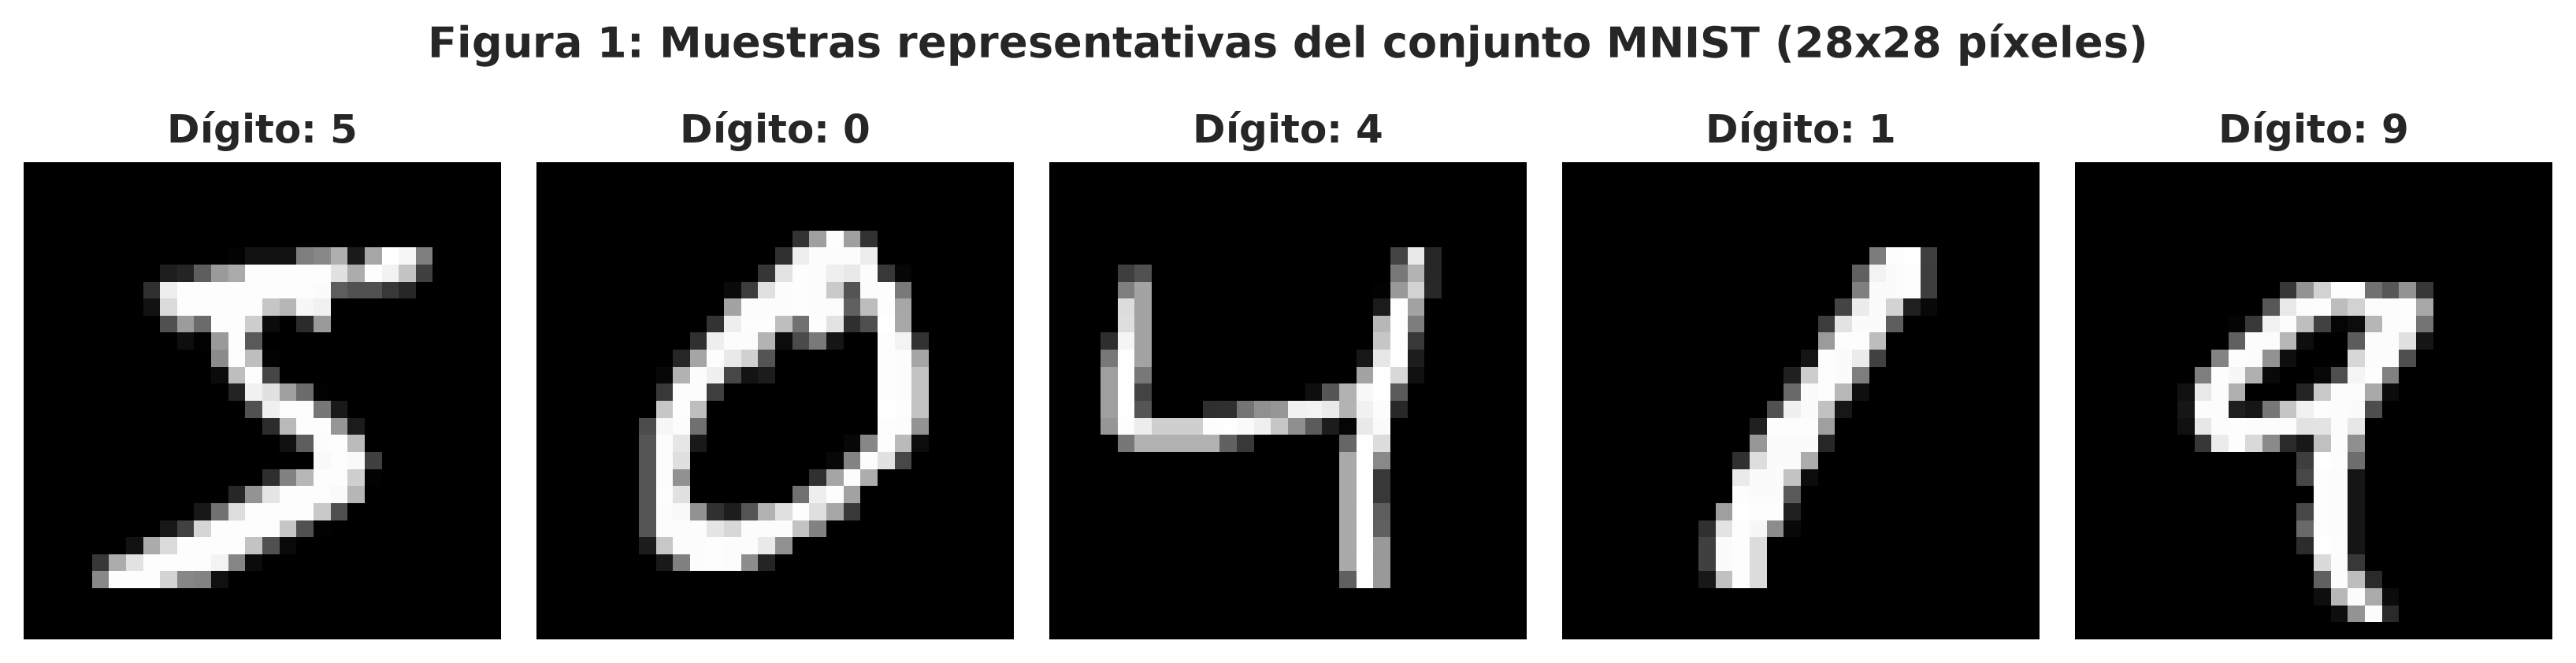
\includegraphics[width=0.88\textwidth]{images/mnist_5_ejemplos.png}
    \caption{Visualización de cinco muestras iniciales del conjunto MNIST y sus etiquetas.}
    \label{fig:ejemplos_mnist}
\end{figure}

En la Tabla~\ref{tab:distribucion} y en la Figura~\ref{fig:distribucion_digitos} se reporta el número exacto de imágenes obtenidas por conjunto y su distribución porcentual por cada dígito ($0$ a $9$), evidenciando el balance estratificado estricto.

\begin{table}[H]
\centering
\caption{Distribución de muestras por dígito en entrenamiento y prueba.}
\label{tab:distribucion}
\small
\renewcommand{\arraystretch}{1.15}
\begin{tabularx}{0.85\textwidth}{>{\centering\arraybackslash}c >{\centering\arraybackslash}X >{\centering\arraybackslash}X >{\centering\arraybackslash}X >{\centering\arraybackslash}X}
\toprule
\textbf{Dígito} & \textbf{Ejemplos Ent.} & \textbf{Prop. Ent. (\%)} & \textbf{Ejemplos Pru.} & \textbf{Prop. Pru. (\%)} \\
\midrule
0 & 987  & 9.87  & 196 & 9.80  \\
1 & 1124 & 11.24 & 227 & 11.35 \\
2 & 993  & 9.93  & 206 & 10.30 \\
3 & 1022 & 10.22 & 202 & 10.10 \\
4 & 974  & 9.74  & 196 & 9.80  \\
5 & 904  & 9.04  & 178 & 8.90  \\
6 & 986  & 9.86  & 192 & 9.60  \\
7 & 1044 & 10.44 & 206 & 10.30 \\
8 & 975  & 9.75  & 195 & 9.75  \\
9 & 991  & 9.91  & 202 & 10.10 \\
\midrule
\textbf{Total} & \textbf{10\,000} & \textbf{100.00\,\%} & \textbf{2\,000} & \textbf{100.00\,\%} \\
\bottomrule
\end{tabularx}
\end{table}

\begin{figure}[H]
    \centering
    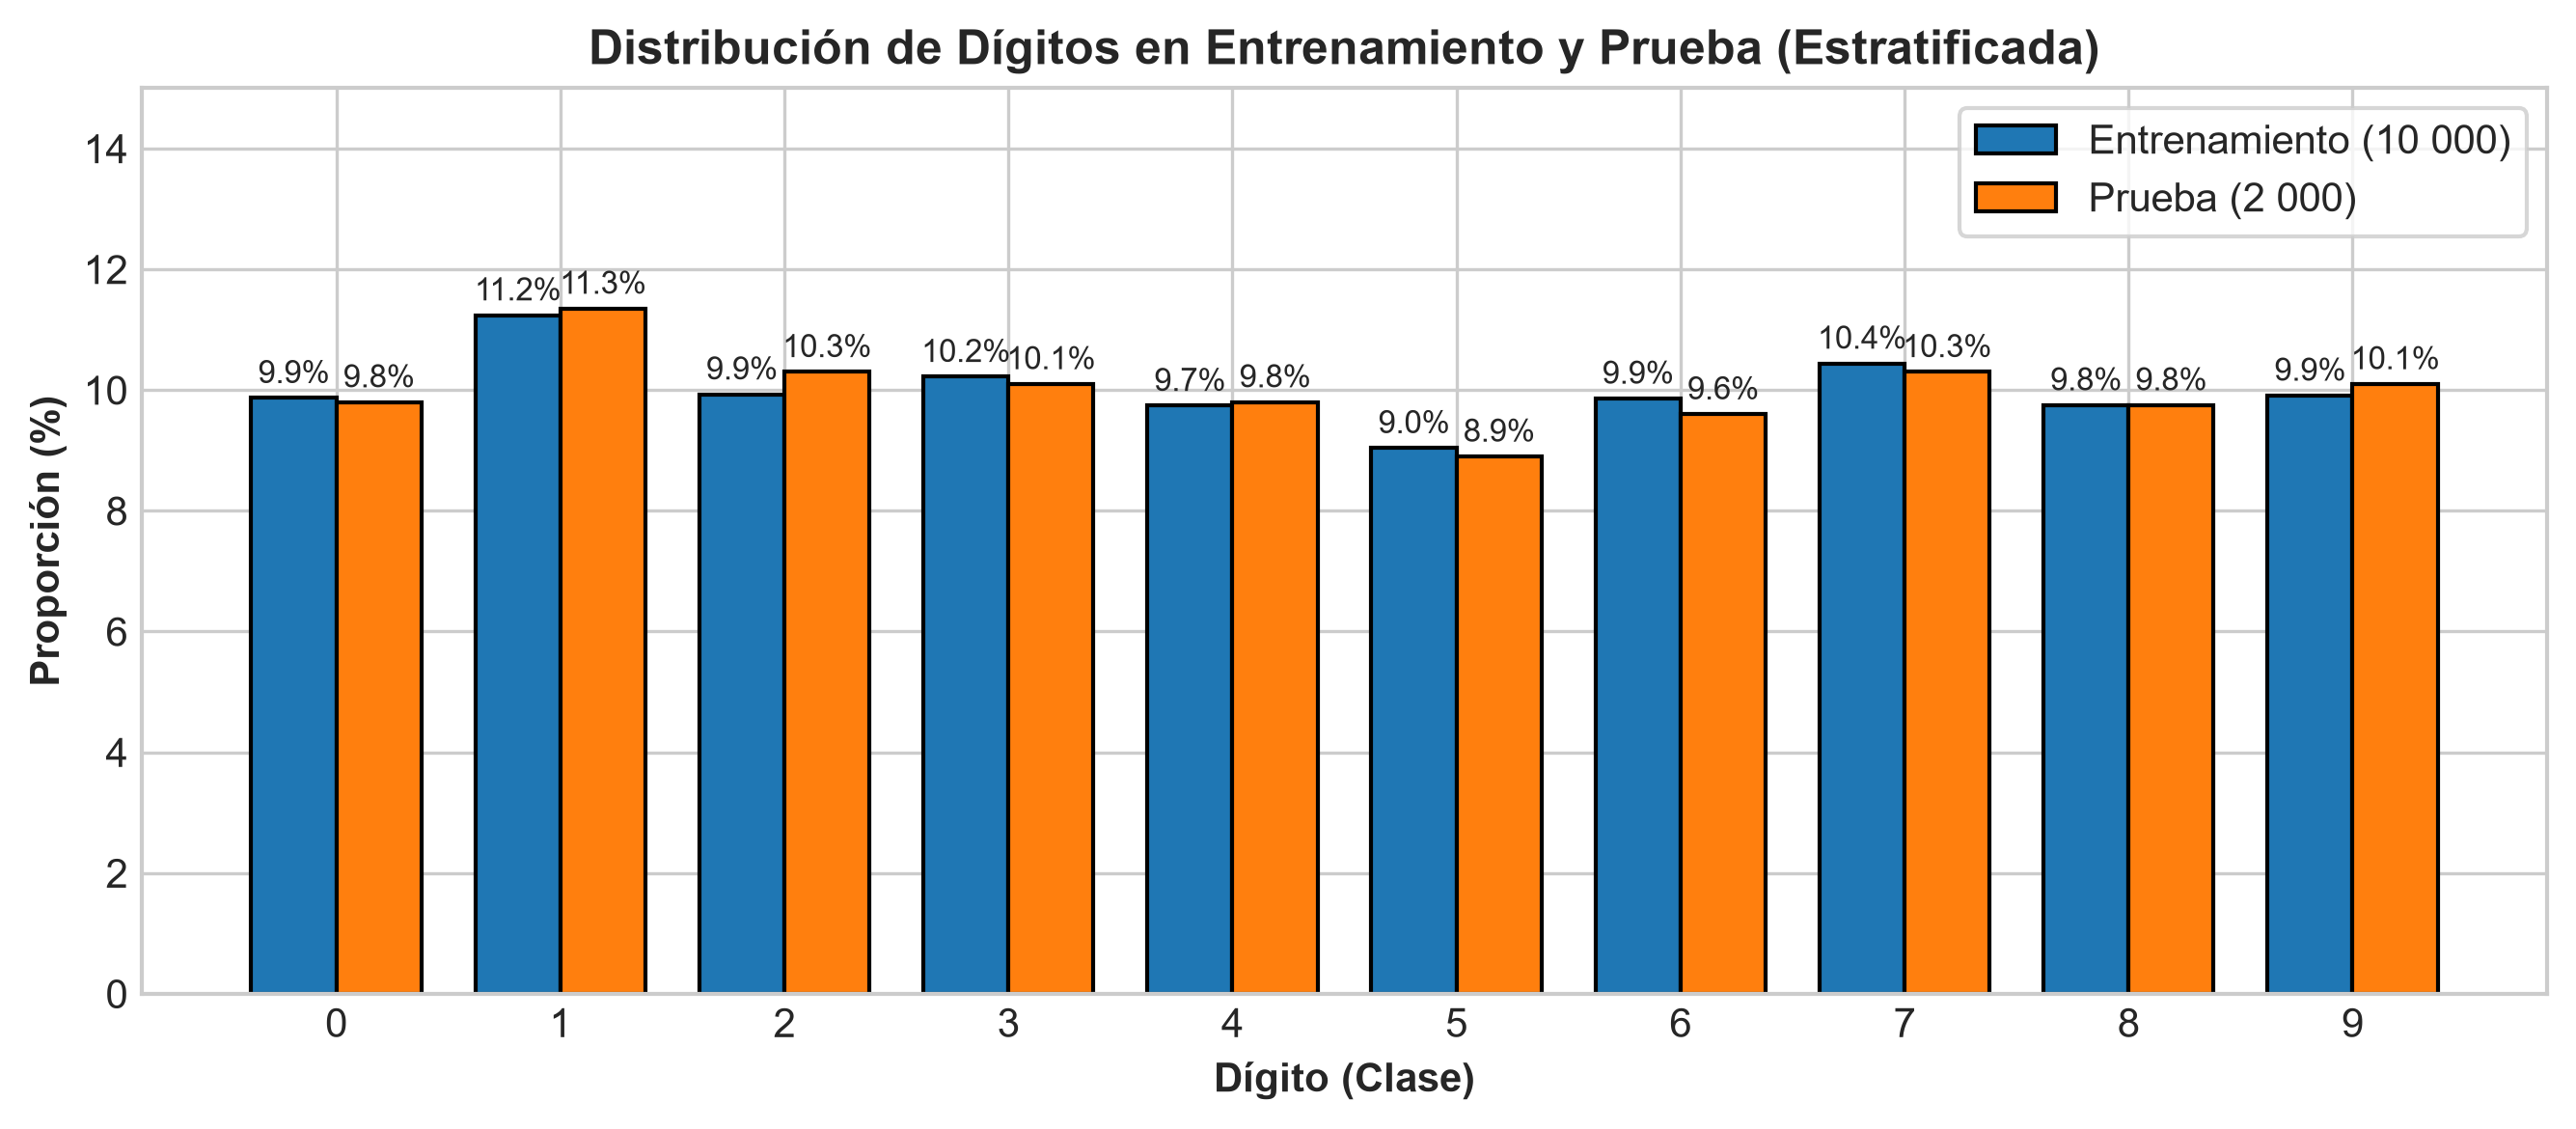
\includegraphics[width=0.75\textwidth]{images/distribucion_digitos.png}
    \caption{Distribución estratificada de dígitos en los conjuntos de entrenamiento ($10\,000$) y prueba ($2\,000$).}
    \label{fig:distribucion_digitos}
\end{figure}

\subsubsection*{2.7.3 Entrenamiento y descripción del funcionamiento de \texttt{fit} (Actividad 2)}
Los tres modelos fueron ajustados exactamente sobre $X_{\text{ent}}$ e $y_{\text{ent}}$. El comportamiento intrínseco de \texttt{fit} en cada clasificador es:
\begin{itemize}[leftmargin=*]
    \item \textbf{Árbol de Decisión:} Al llamar \texttt{fit}, el algoritmo construye recursivamente un árbol binario calculando en cada nodo la característica de píxel y el umbral escalar que maximicen la reducción de impureza de Gini:
    \[
    I_G(D) = 1 - \sum_{k=0}^{9} p_k^2
    \]
    El árbol crece hasta alcanzar la cota restrictiva fijada de 15 niveles de profundidad (\texttt{max\_depth=15}). Tiempo de ajuste: \textbf{4.94 segundos}.
    
    \item \textbf{Random Forest:} Durante \texttt{fit}, genera un ensamble constituido por 100 árboles de decisión independientes (\texttt{n\_estimators=100}). Cada árbol individual se entrena con una muestra generada mediante remuestreo con reemplazo (\textit{bootstrap}) del conjunto de entrenamiento y, en cada bifurcación, evalúa únicamente un subconjunto aleatorio de variables ($m = \lfloor \sqrt{784} \rfloor = 28$ píxeles), mitigando drásticamente la correlación entre árboles y la varianza del ensamble:
    \[
    \text{Var}\left( \frac{1}{B}\sum_{b=1}^B T_b(x) \right) = \rho \sigma^2 + \frac{1 - \rho}{B}\sigma^2
    \]
    Tiempo de ajuste: \textbf{11.70 segundos}.
    
    \item \textbf{k-NN (k-Nearest Neighbors):} Al ser un algoritmo de aprendizaje perezoso (\textit{lazy learning}), el método \texttt{fit} no calcula coeficientes paramétricos analíticos; únicamente indexa los 10\,000 vectores en estructuras jerárquicas espaciales (KD-Tree/Ball-Tree) en memoria para permitir consultas de distancia euclidiana durante la inferencia. Tiempo de ajuste: \textbf{0.01 segundos}.
\end{itemize}

\subsubsection*{2.7.4 Resultados de evaluación en entrenamiento y prueba (Actividad 3)}
Las predicciones se obtuvieron aplicando \texttt{predict} de forma independiente sobre entrenamiento y prueba. En la Tabla~\ref{tab:resultados_ent_pru} se presentan los resultados con dos decimales exactos.

\begin{table}[H]
\centering
\caption{Resultados de evaluación en entrenamiento y prueba (Tabla 2 de la guía).}
\label{tab:resultados_ent_pru}
\renewcommand{\arraystretch}{1.25}
\begin{tabularx}{\textwidth}{l >{\centering\arraybackslash}X >{\centering\arraybackslash}X >{\centering\arraybackslash}X >{\centering\arraybackslash}X >{\centering\arraybackslash}X}
\toprule
\textbf{Modelo} & \textbf{Exactitud ent. (\%)} & \textbf{Error ent. (\%)} & \textbf{Exactitud prueba (\%)} & \textbf{Error prueba (\%)} & \textbf{Brecha (p. p.)} \\
\midrule
Árbol de decisión & 99.02 & 0.98 & 81.80 & 18.20 & 17.22 \\
Random Forest     & 99.93 & 0.07 & 94.80 & 5.20  & 5.13  \\
k-NN              & 96.51 & 3.49 & 94.55 & 5.45  & 1.96  \\
\bottomrule
\end{tabularx}
\begin{flushleft}
\footnotesize \textit{Nota:} Ent. = entrenamiento; p. p. = puntos porcentuales. Se verificó que en cada conjunto la exactitud y el error sumen exactamente el 100.00\,\%.
\end{flushleft}
\end{table}

En la Figura~\ref{fig:comparativa_metricas} se muestra la comparativa visual de exactitud y brecha de sobreajuste, mientras que en la Figura~\ref{fig:comparativa_tiempos} se ilustra el análisis computacional de tiempos de entrenamiento e inferencia en escala logarítmica.

\begin{figure}[H]
    \centering
    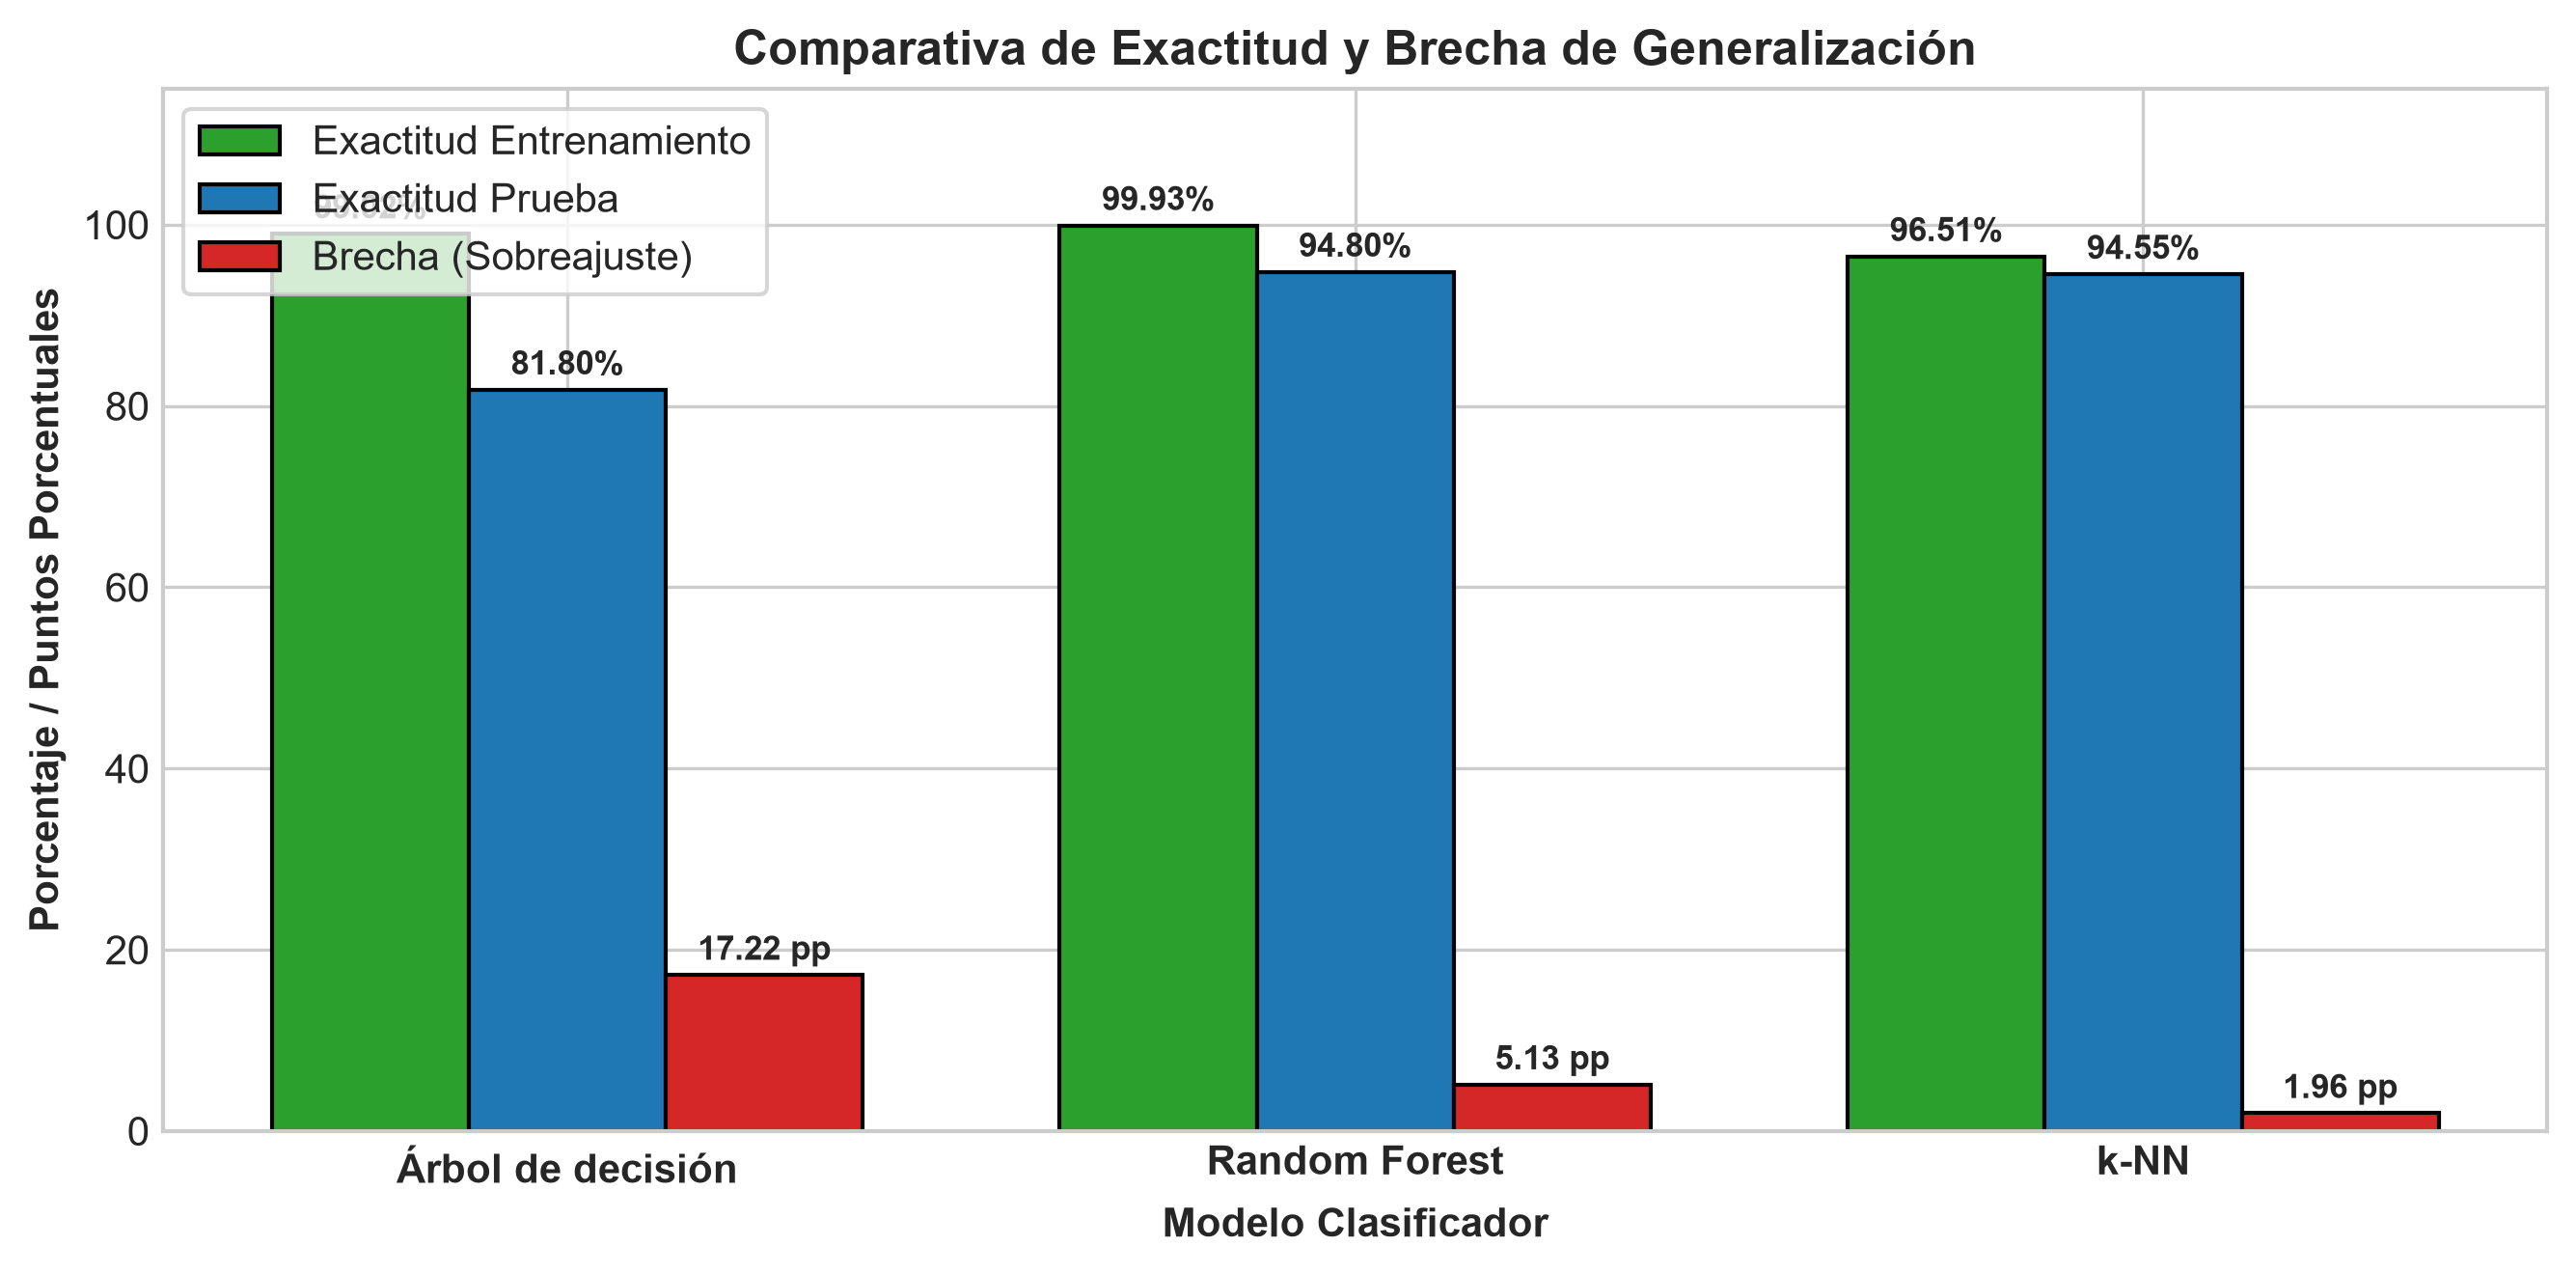
\includegraphics[width=0.82\textwidth]{images/comparativa_metricas.png}
    \caption{Comparativa cuantitativa de exactitud en entrenamiento vs prueba y brecha de sobreajuste.}
    \label{fig:comparativa_metricas}
\end{figure}

\begin{figure}[H]
    \centering
    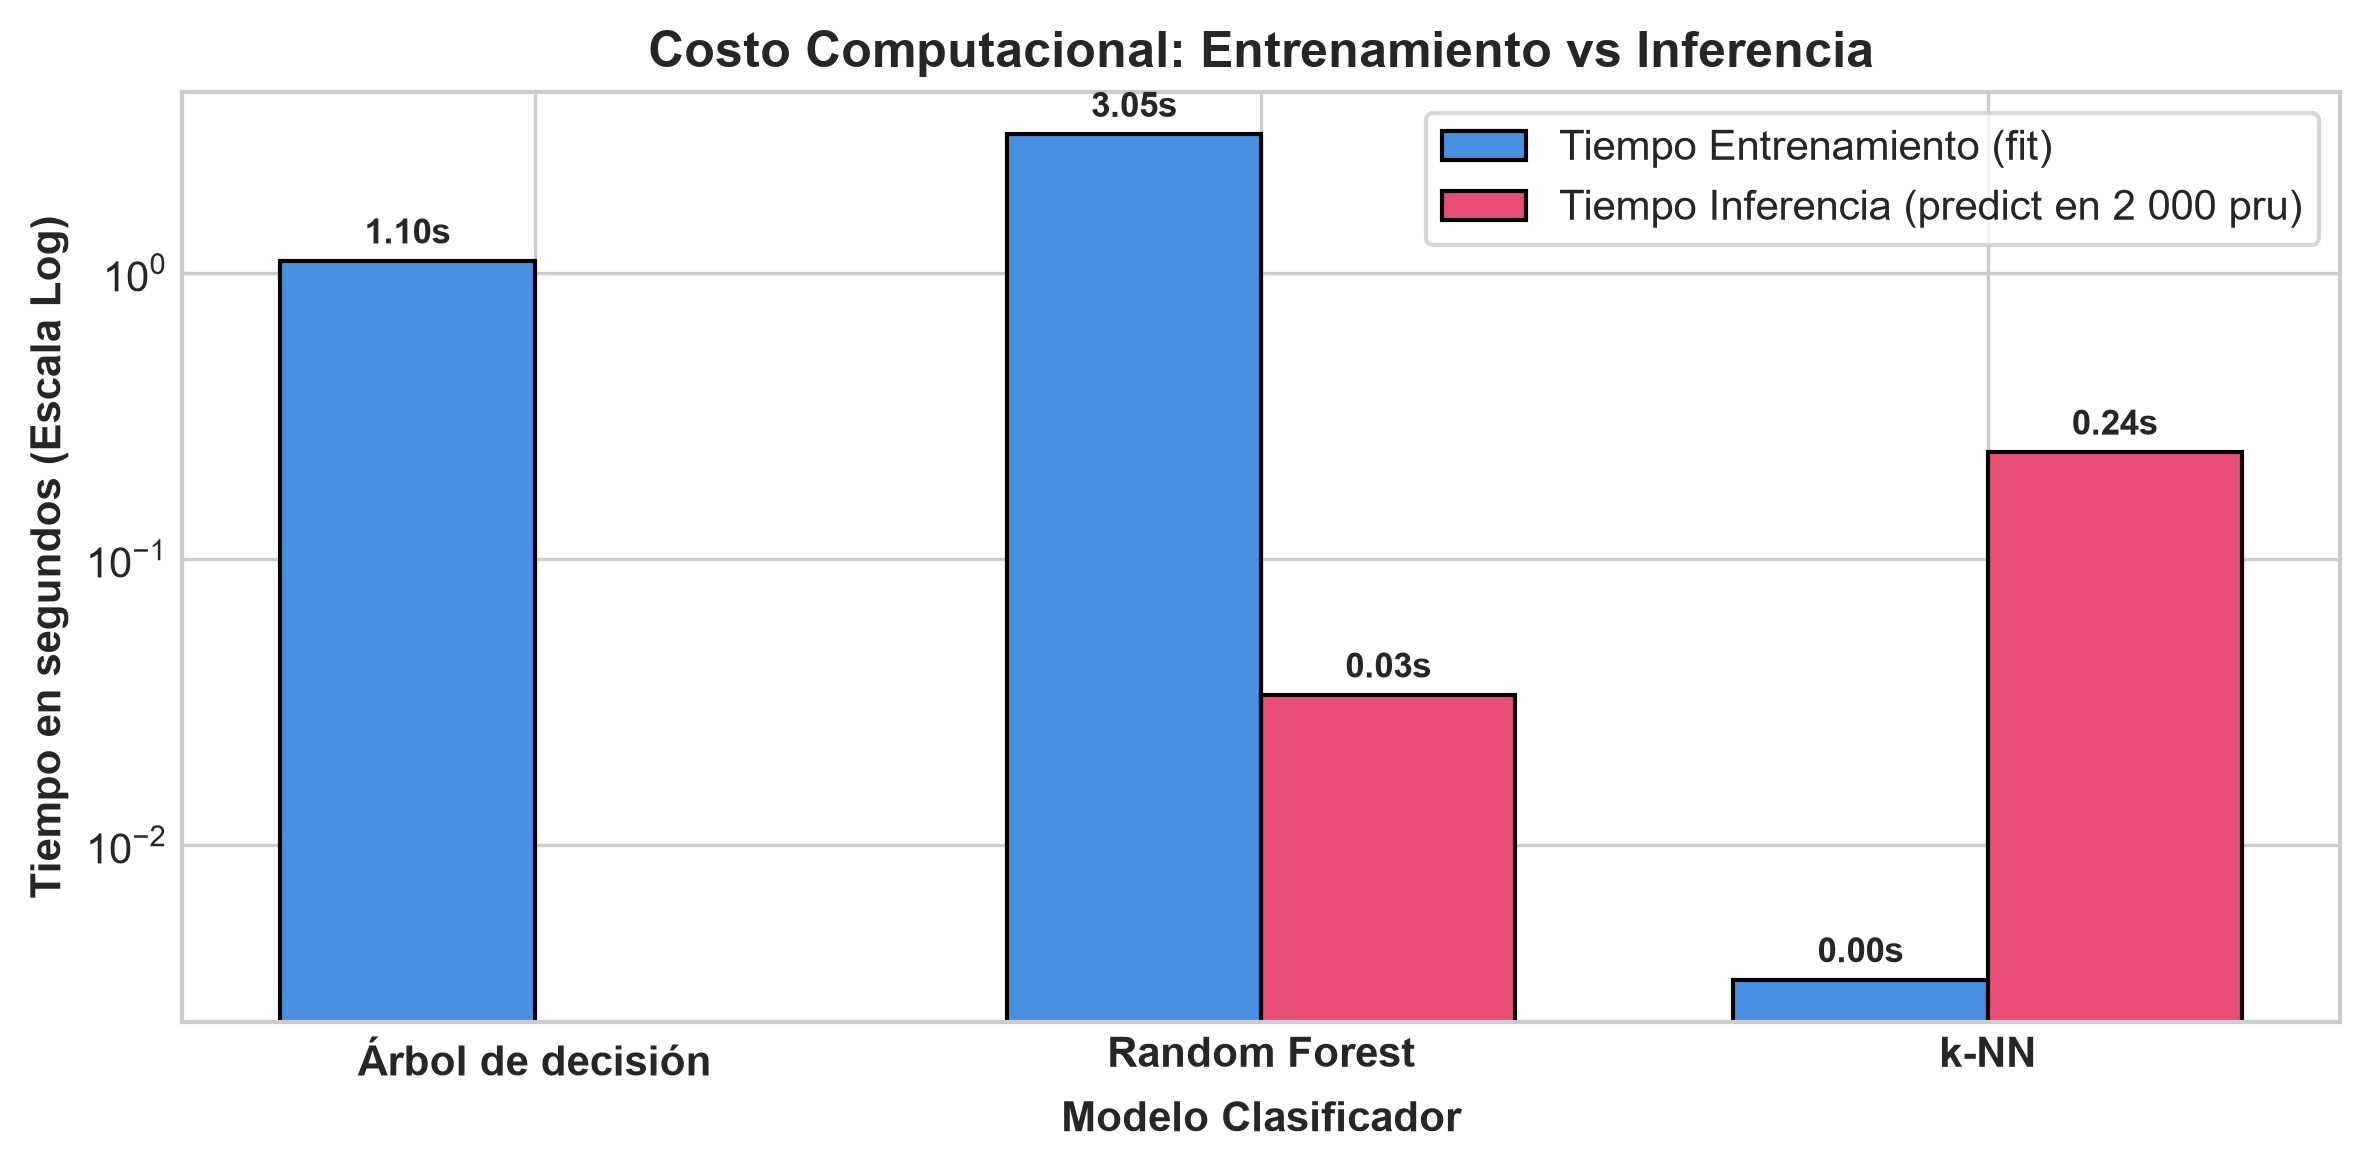
\includegraphics[width=0.78\textwidth]{images/comparativa_tiempos.png}
    \caption{Costo computacional de entrenamiento e inferencia en escala logarítmica para los tres clasificadores.}
    \label{fig:comparativa_tiempos}
\end{figure}

\subsubsection*{2.7.5 Matrices de confusión y análisis de errores (Actividad 4)}
En la Figura~\ref{fig:matrices_confusion_comparativa} se exhiben las tres matrices de confusión de prueba ($2\,000$ ejemplos) obtenidas para cada clasificador. En la Figura~\ref{fig:matrices_individuales} se presentan adicionalmente de forma individual con escala de color y valores enteros.

\begin{figure}[H]
    \centering
    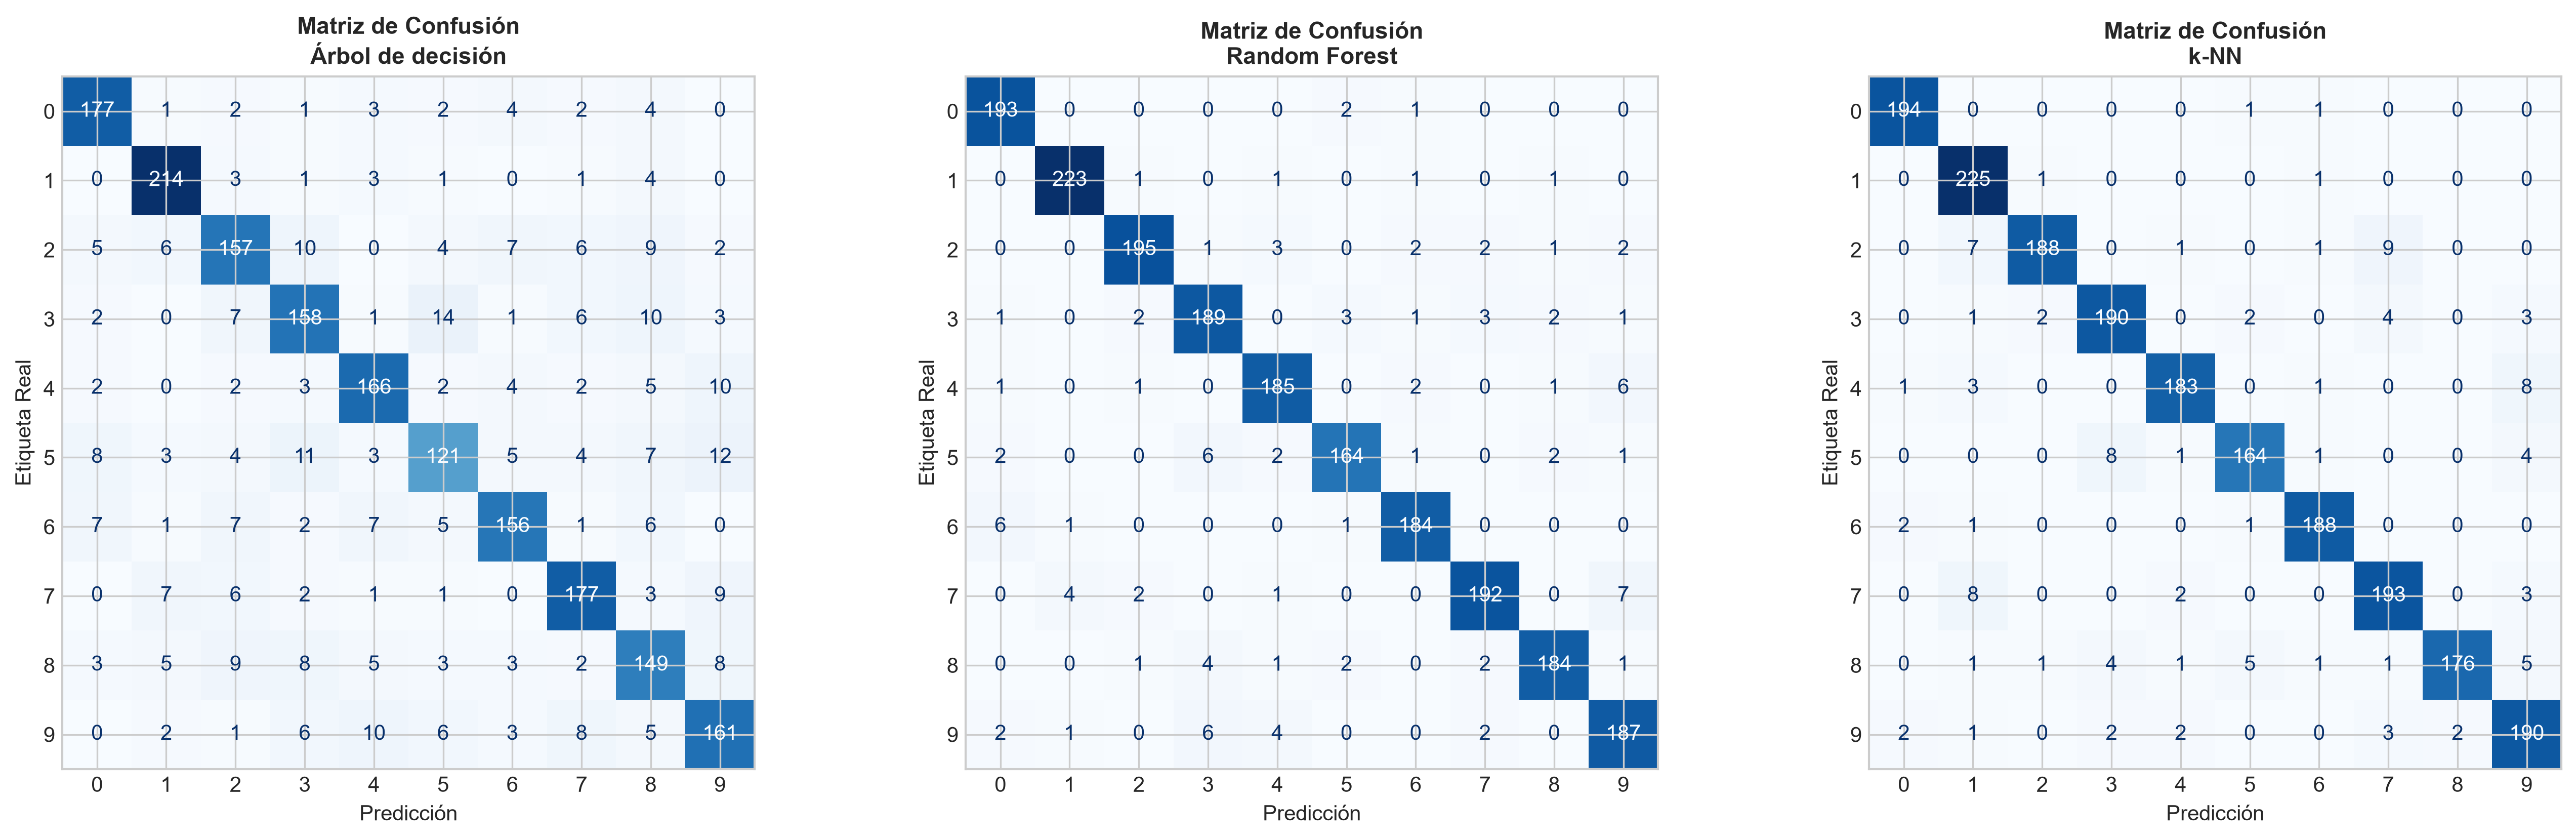
\includegraphics[width=\textwidth]{images/matrices_confusion_comparativa.png}
    \caption{Matrices de confusión sobre el conjunto de prueba ($2\,000$ ejemplos) para Árbol de Decisión, Random Forest y k-NN.}
    \label{fig:matrices_confusion_comparativa}
\end{figure}

\begin{figure}[H]
    \centering
    \begin{subfigure}[b]{0.32\textwidth}
        \centering
        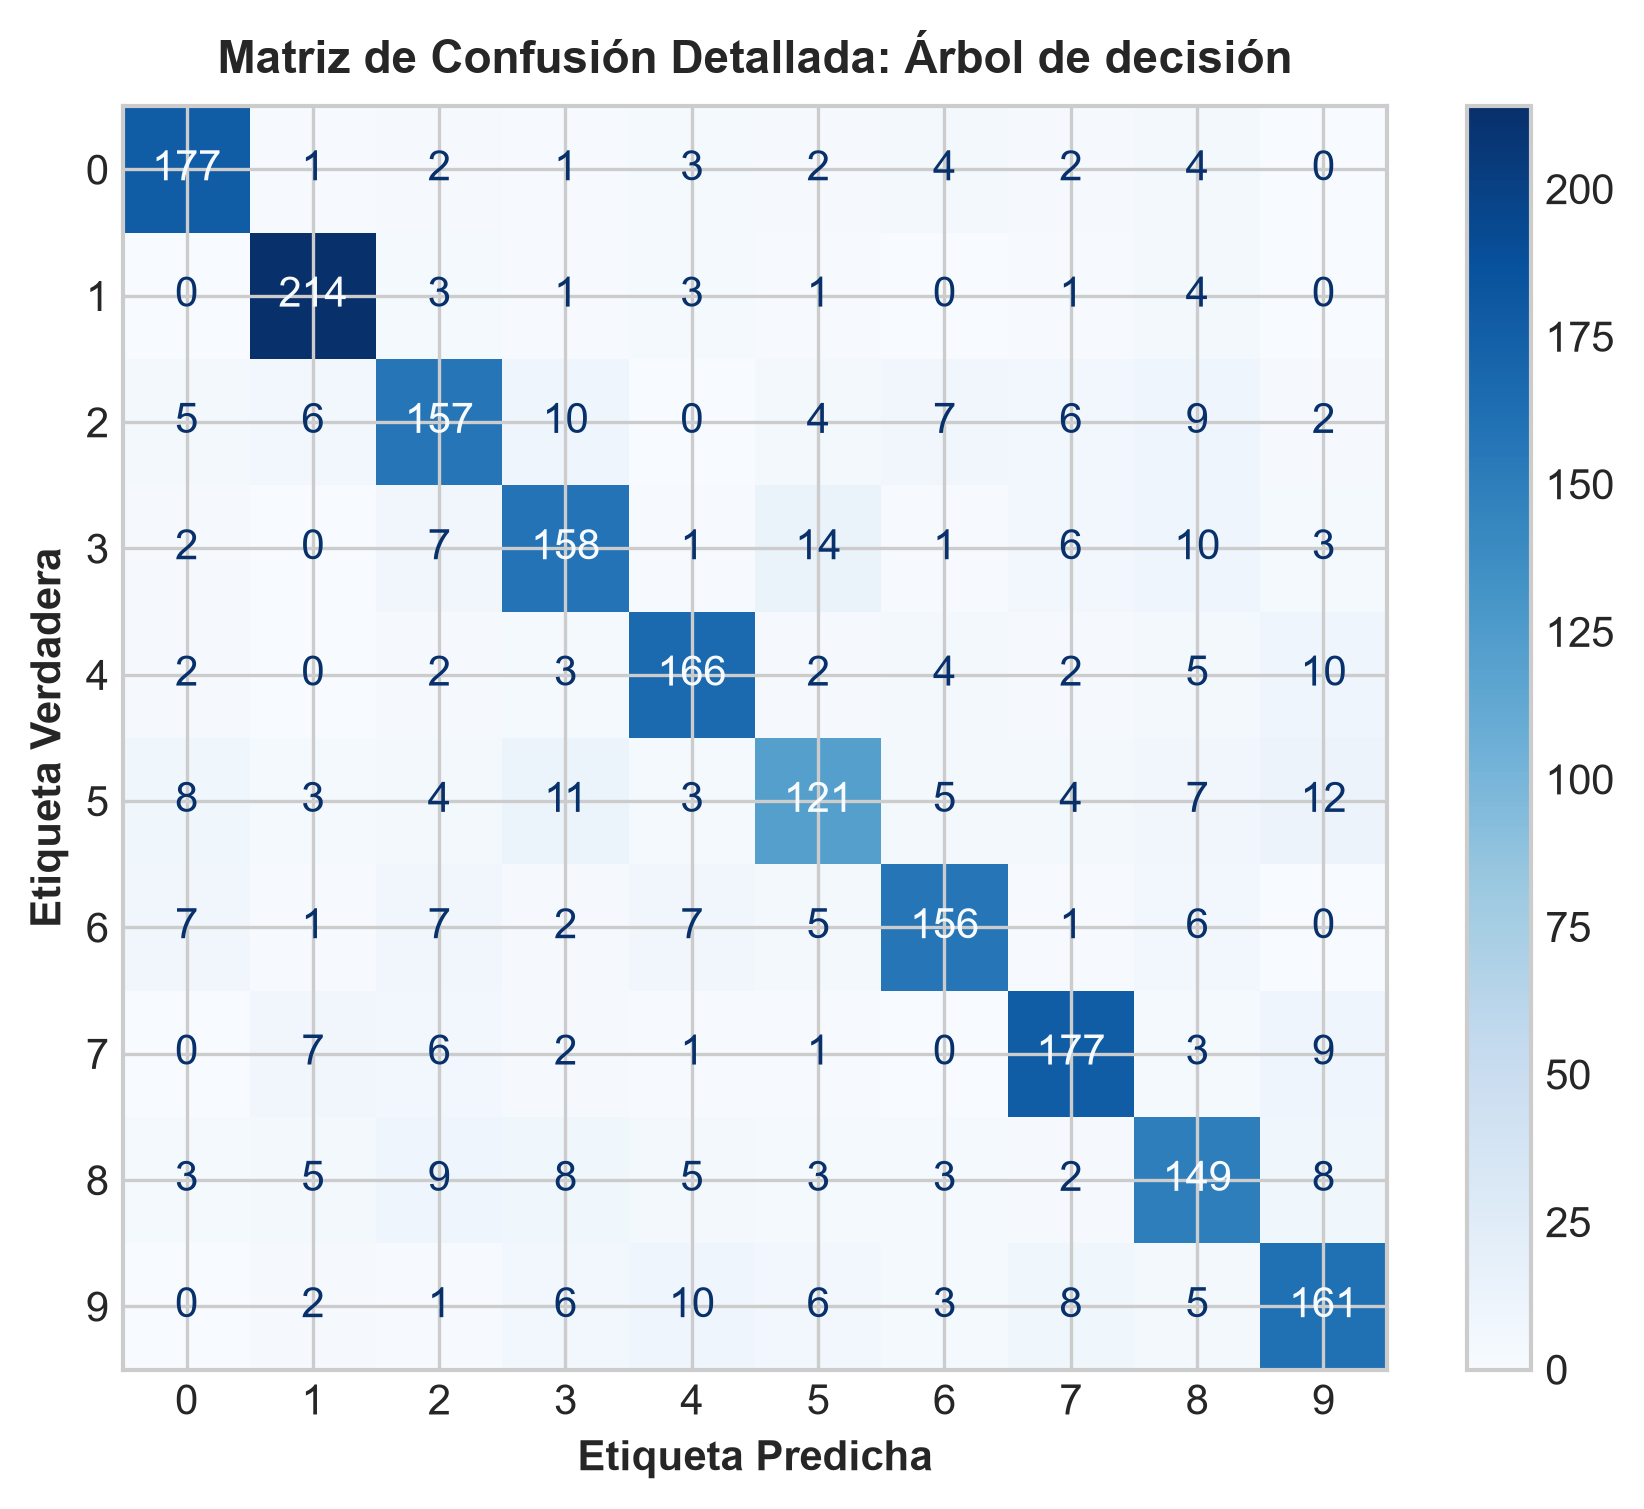
\includegraphics[width=\textwidth]{images/cm_arbol_de_decision.png}
        \caption{Árbol de Decisión}
    \end{subfigure}
    \hfill
    \begin{subfigure}[b]{0.32\textwidth}
        \centering
        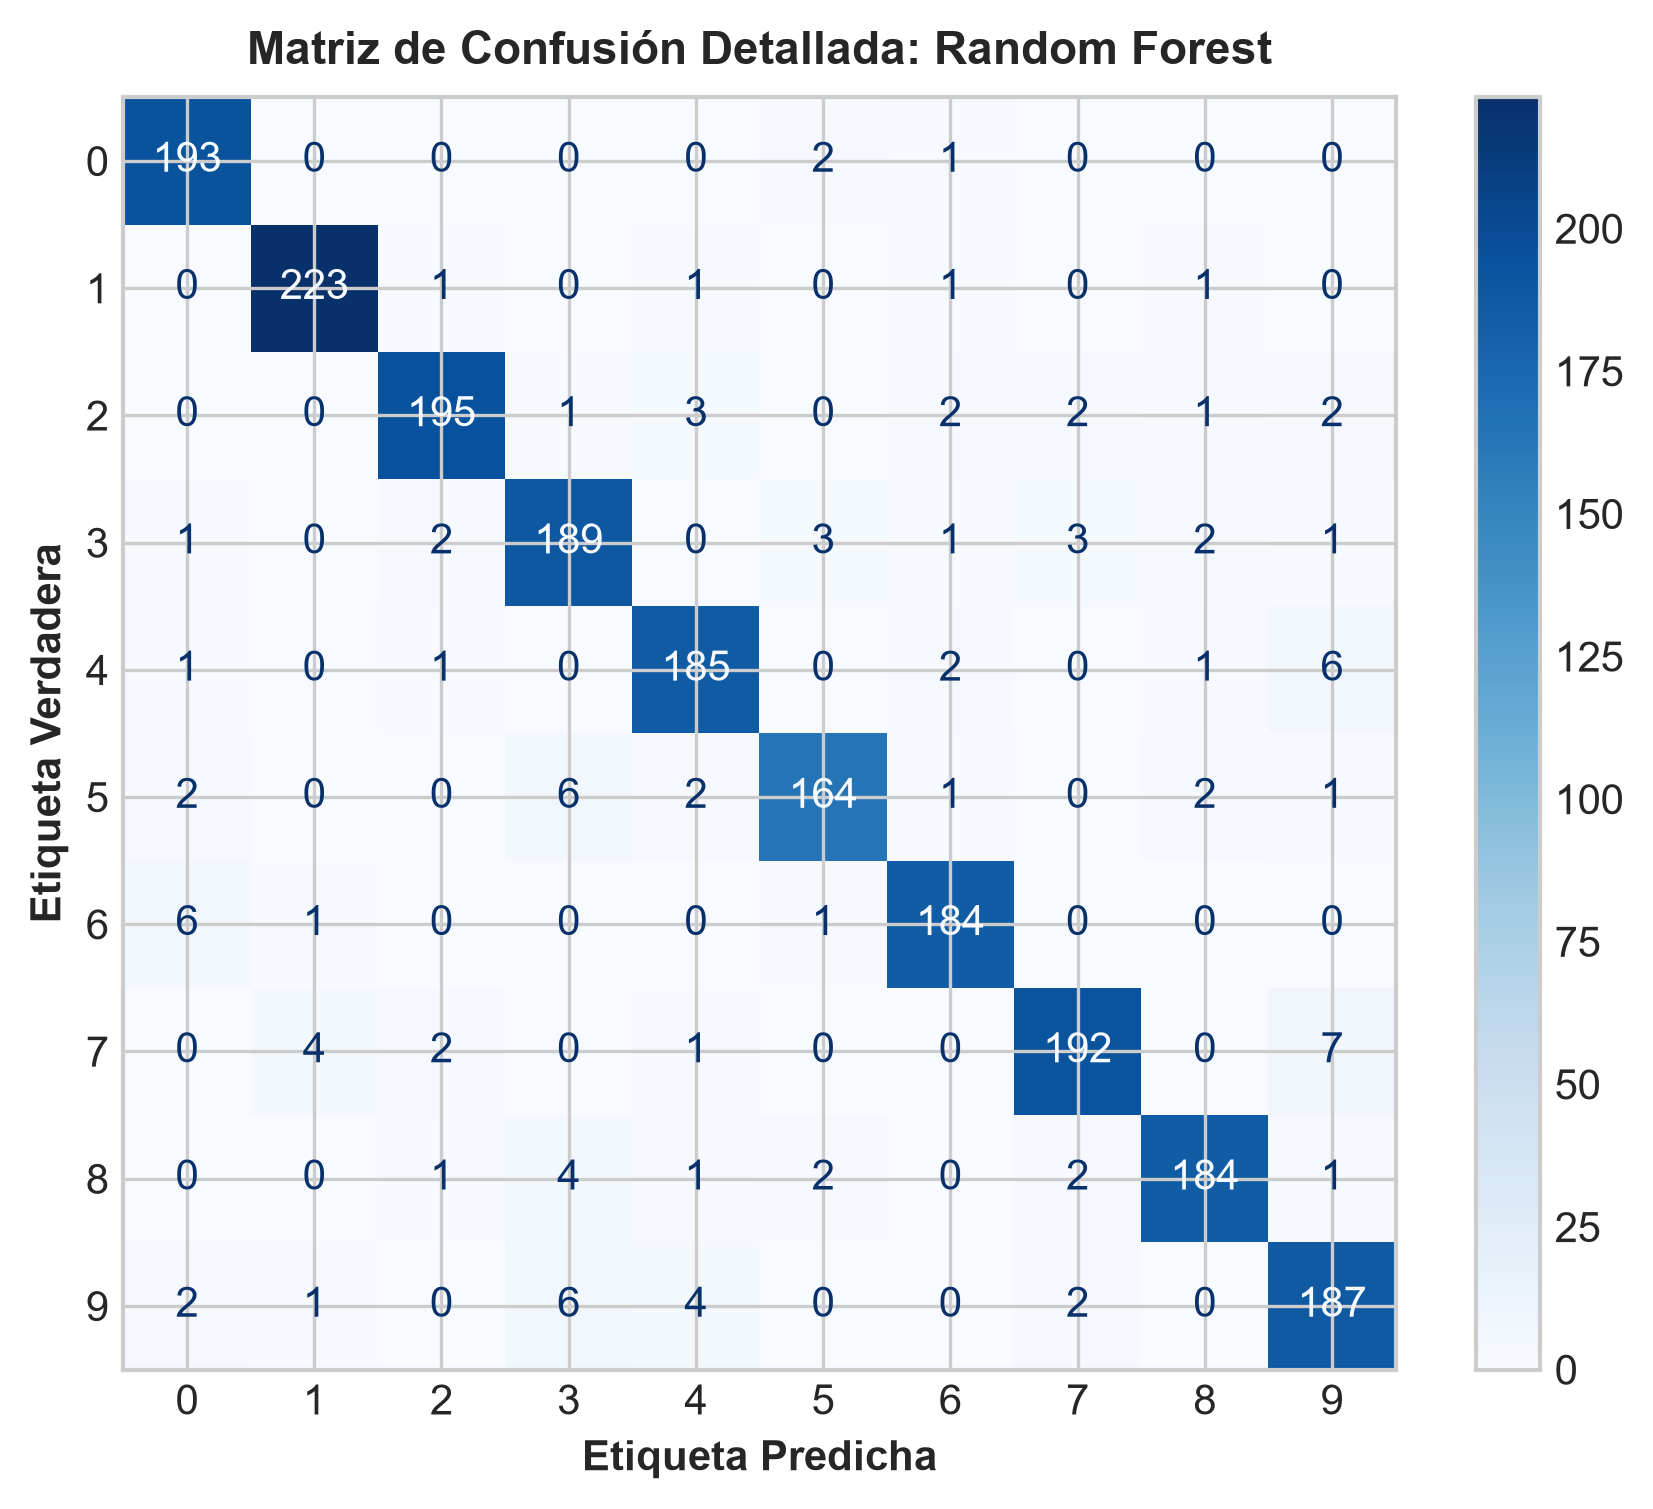
\includegraphics[width=\textwidth]{images/cm_random_forest.png}
        \caption{Random Forest}
    \end{subfigure}
    \hfill
    \begin{subfigure}[b]{0.32\textwidth}
        \centering
        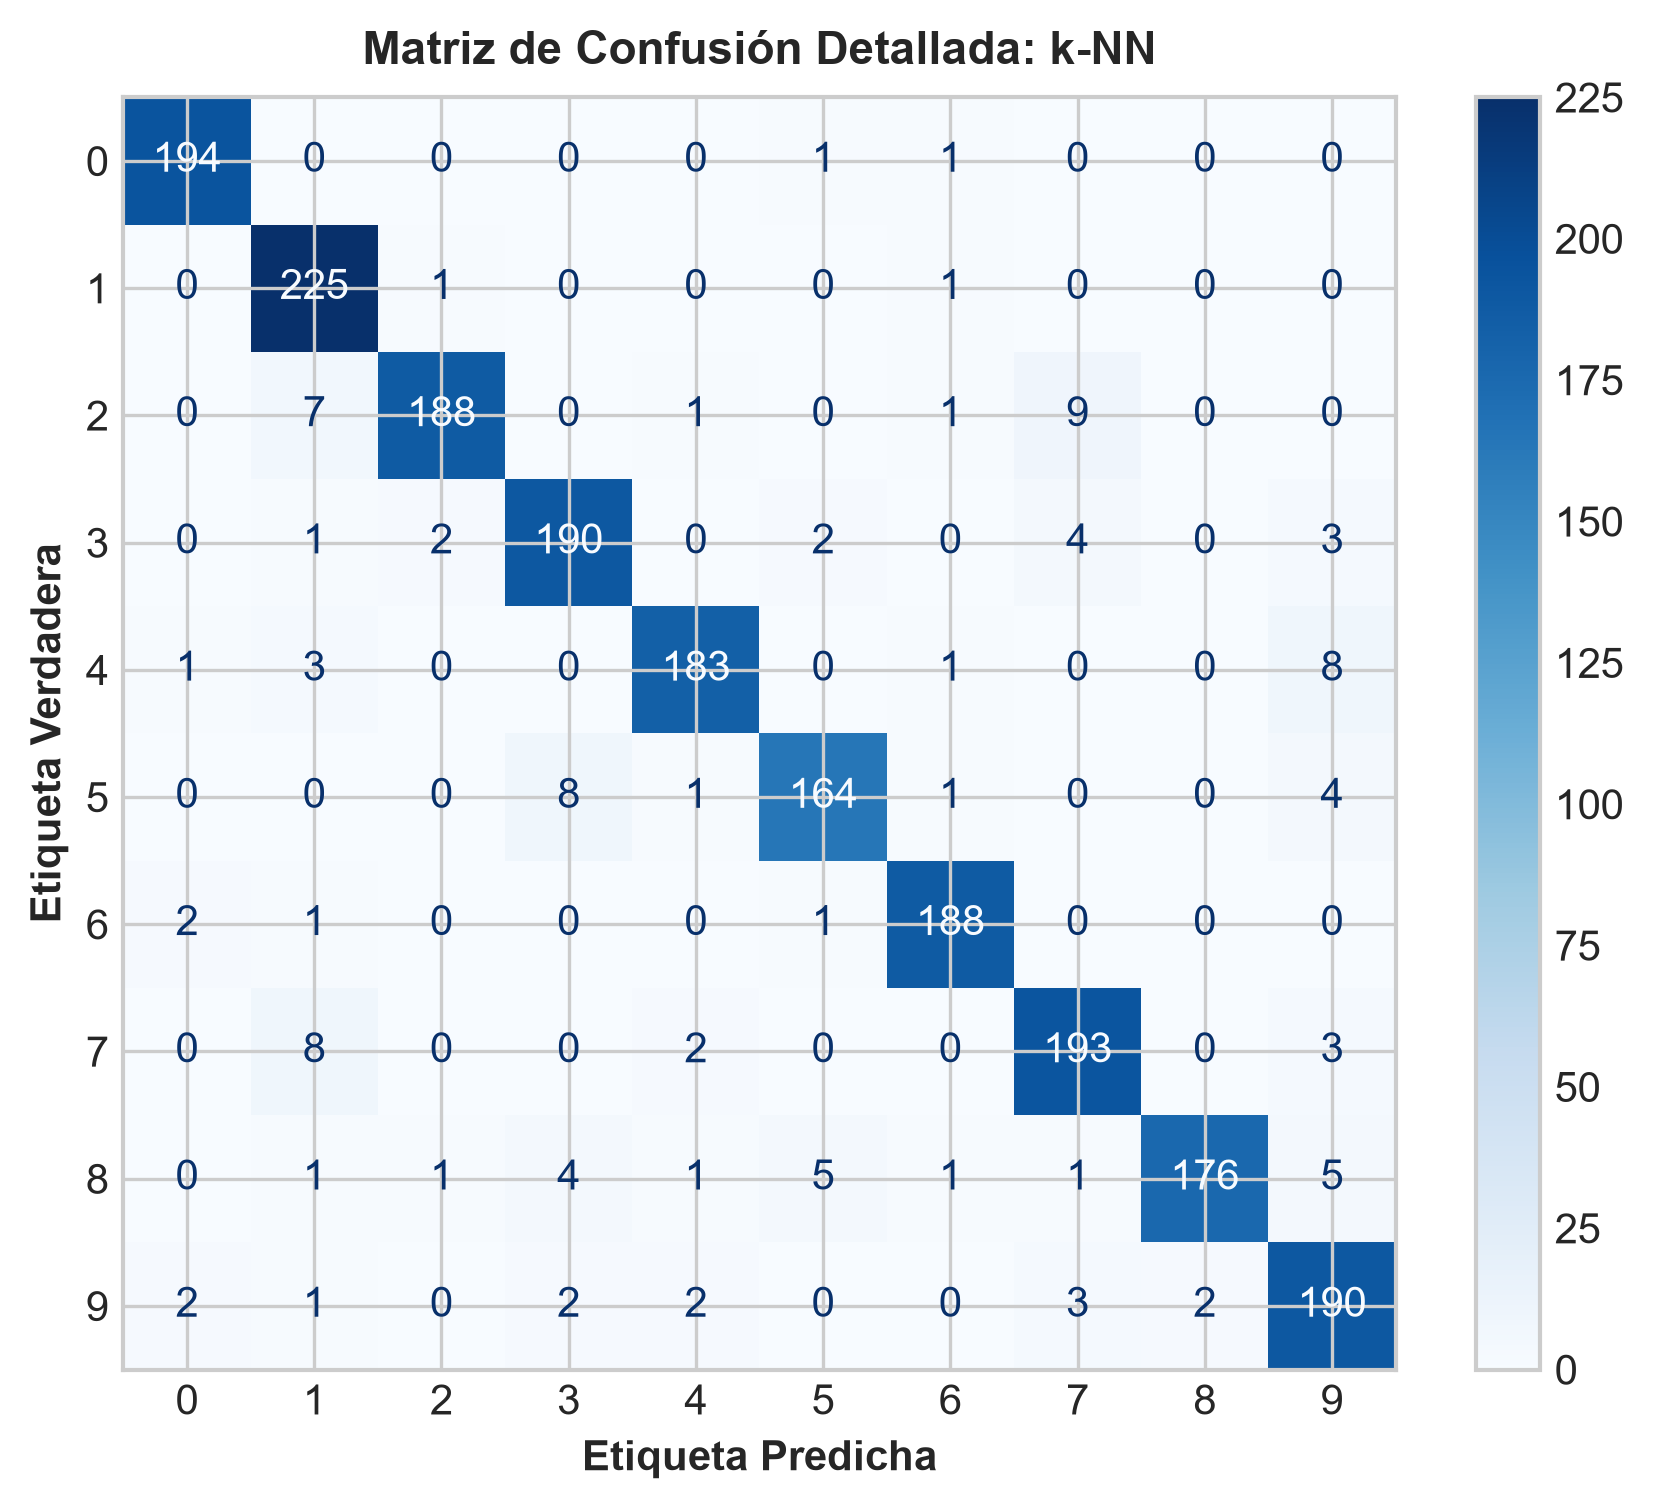
\includegraphics[width=\textwidth]{images/cm_knn.png}
        \caption{k-NN ($k=5$)}
    \end{subfigure}
    \caption{Matrices de confusión individuales detalladas con valores cuantitativos por celda.}
    \label{fig:matrices_individuales}
\end{figure}

\paragraph{Confusiones más frecuentes entre dígitos distintos ($i \neq j$):}
\begin{itemize}[leftmargin=*]
    \item \textbf{Árbol de decisión:} La confusión más frecuente se suscitó entre el \textbf{dígito real 3 clasificado erróneamente como 5}, registrando un total de \textbf{14 casos} (seguido por 4 vs 9 con 11 casos y 7 vs 9 con 11 casos).
    \item \textbf{Random Forest:} La confusión más frecuente ocurrió entre el \textbf{dígito real 7 clasificado erróneamente como 9}, registrando un total de \textbf{7 casos}.
    \item \textbf{k-NN:} La confusión más frecuente se dio entre el \textbf{dígito real 2 clasificado erróneamente como 7}, alcanzando \textbf{9 casos}.
\end{itemize}

\paragraph{Muestra de prueba mal clasificada:}
En la Figura~\ref{fig:ejemplo_error} se expone la muestra de prueba \#64 (etiqueta real 2), en la cual el Árbol predijo 6, Random Forest predijo 4, y k-NN acertó correctamente prediciendo 2. En la Figura~\ref{fig:galeria_errores} se complementa el estudio con una galería de 6 casos de prueba representativos con trazos ambiguos.

\begin{figure}[H]
    \centering
    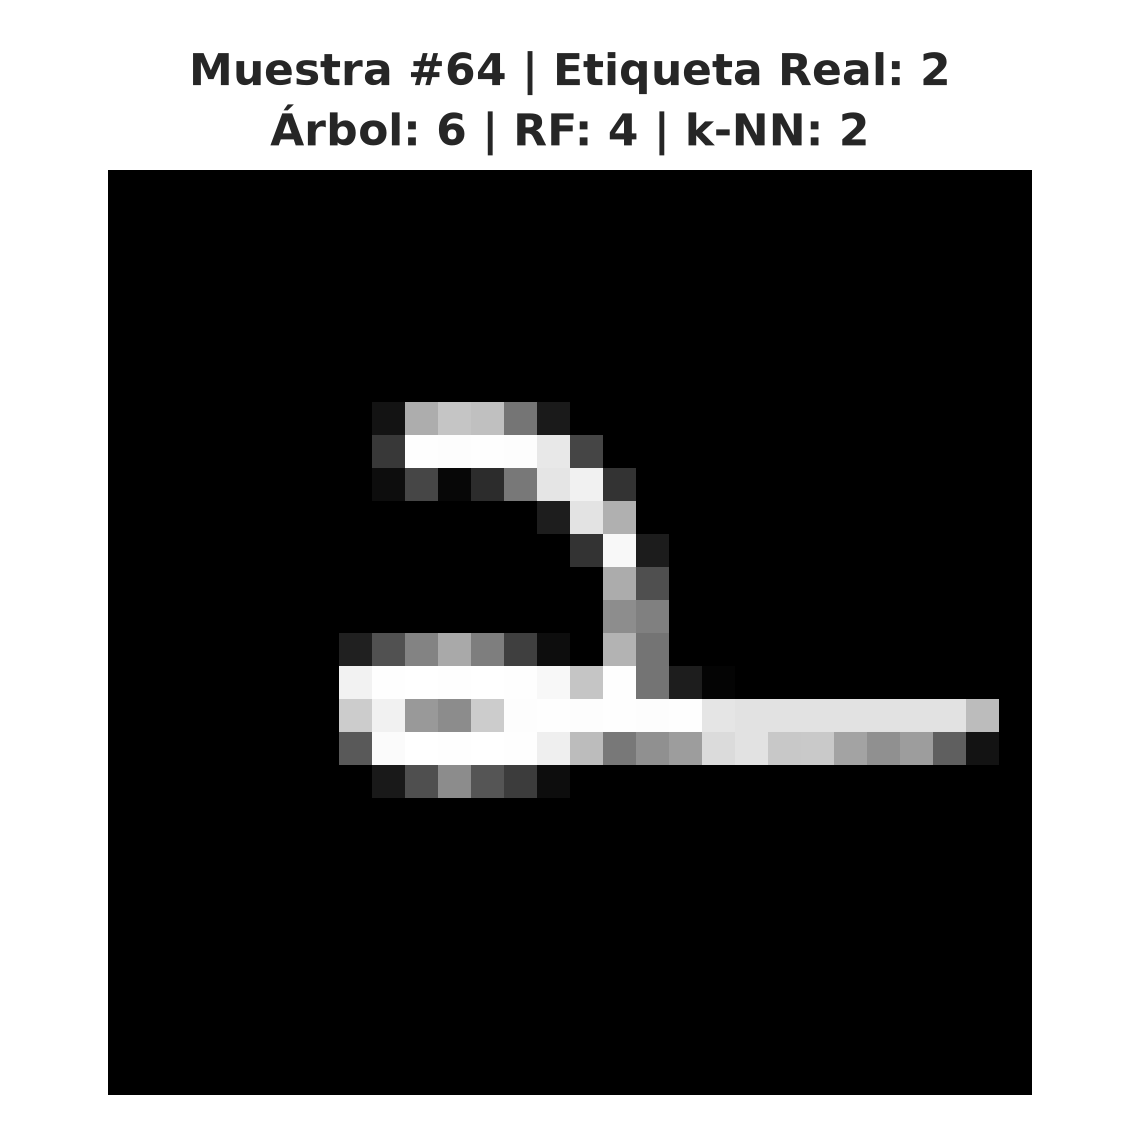
\includegraphics[width=0.32\textwidth]{images/ejemplo_mal_clasificado.png}
    \caption{Muestra de prueba \#64 con caligrafía atípica: etiqueta real 2, predicciones: Árbol=6, Random Forest=4, k-NN=2.}
    \label{fig:ejemplo_error}
\end{figure}

\begin{figure}[H]
    \centering
    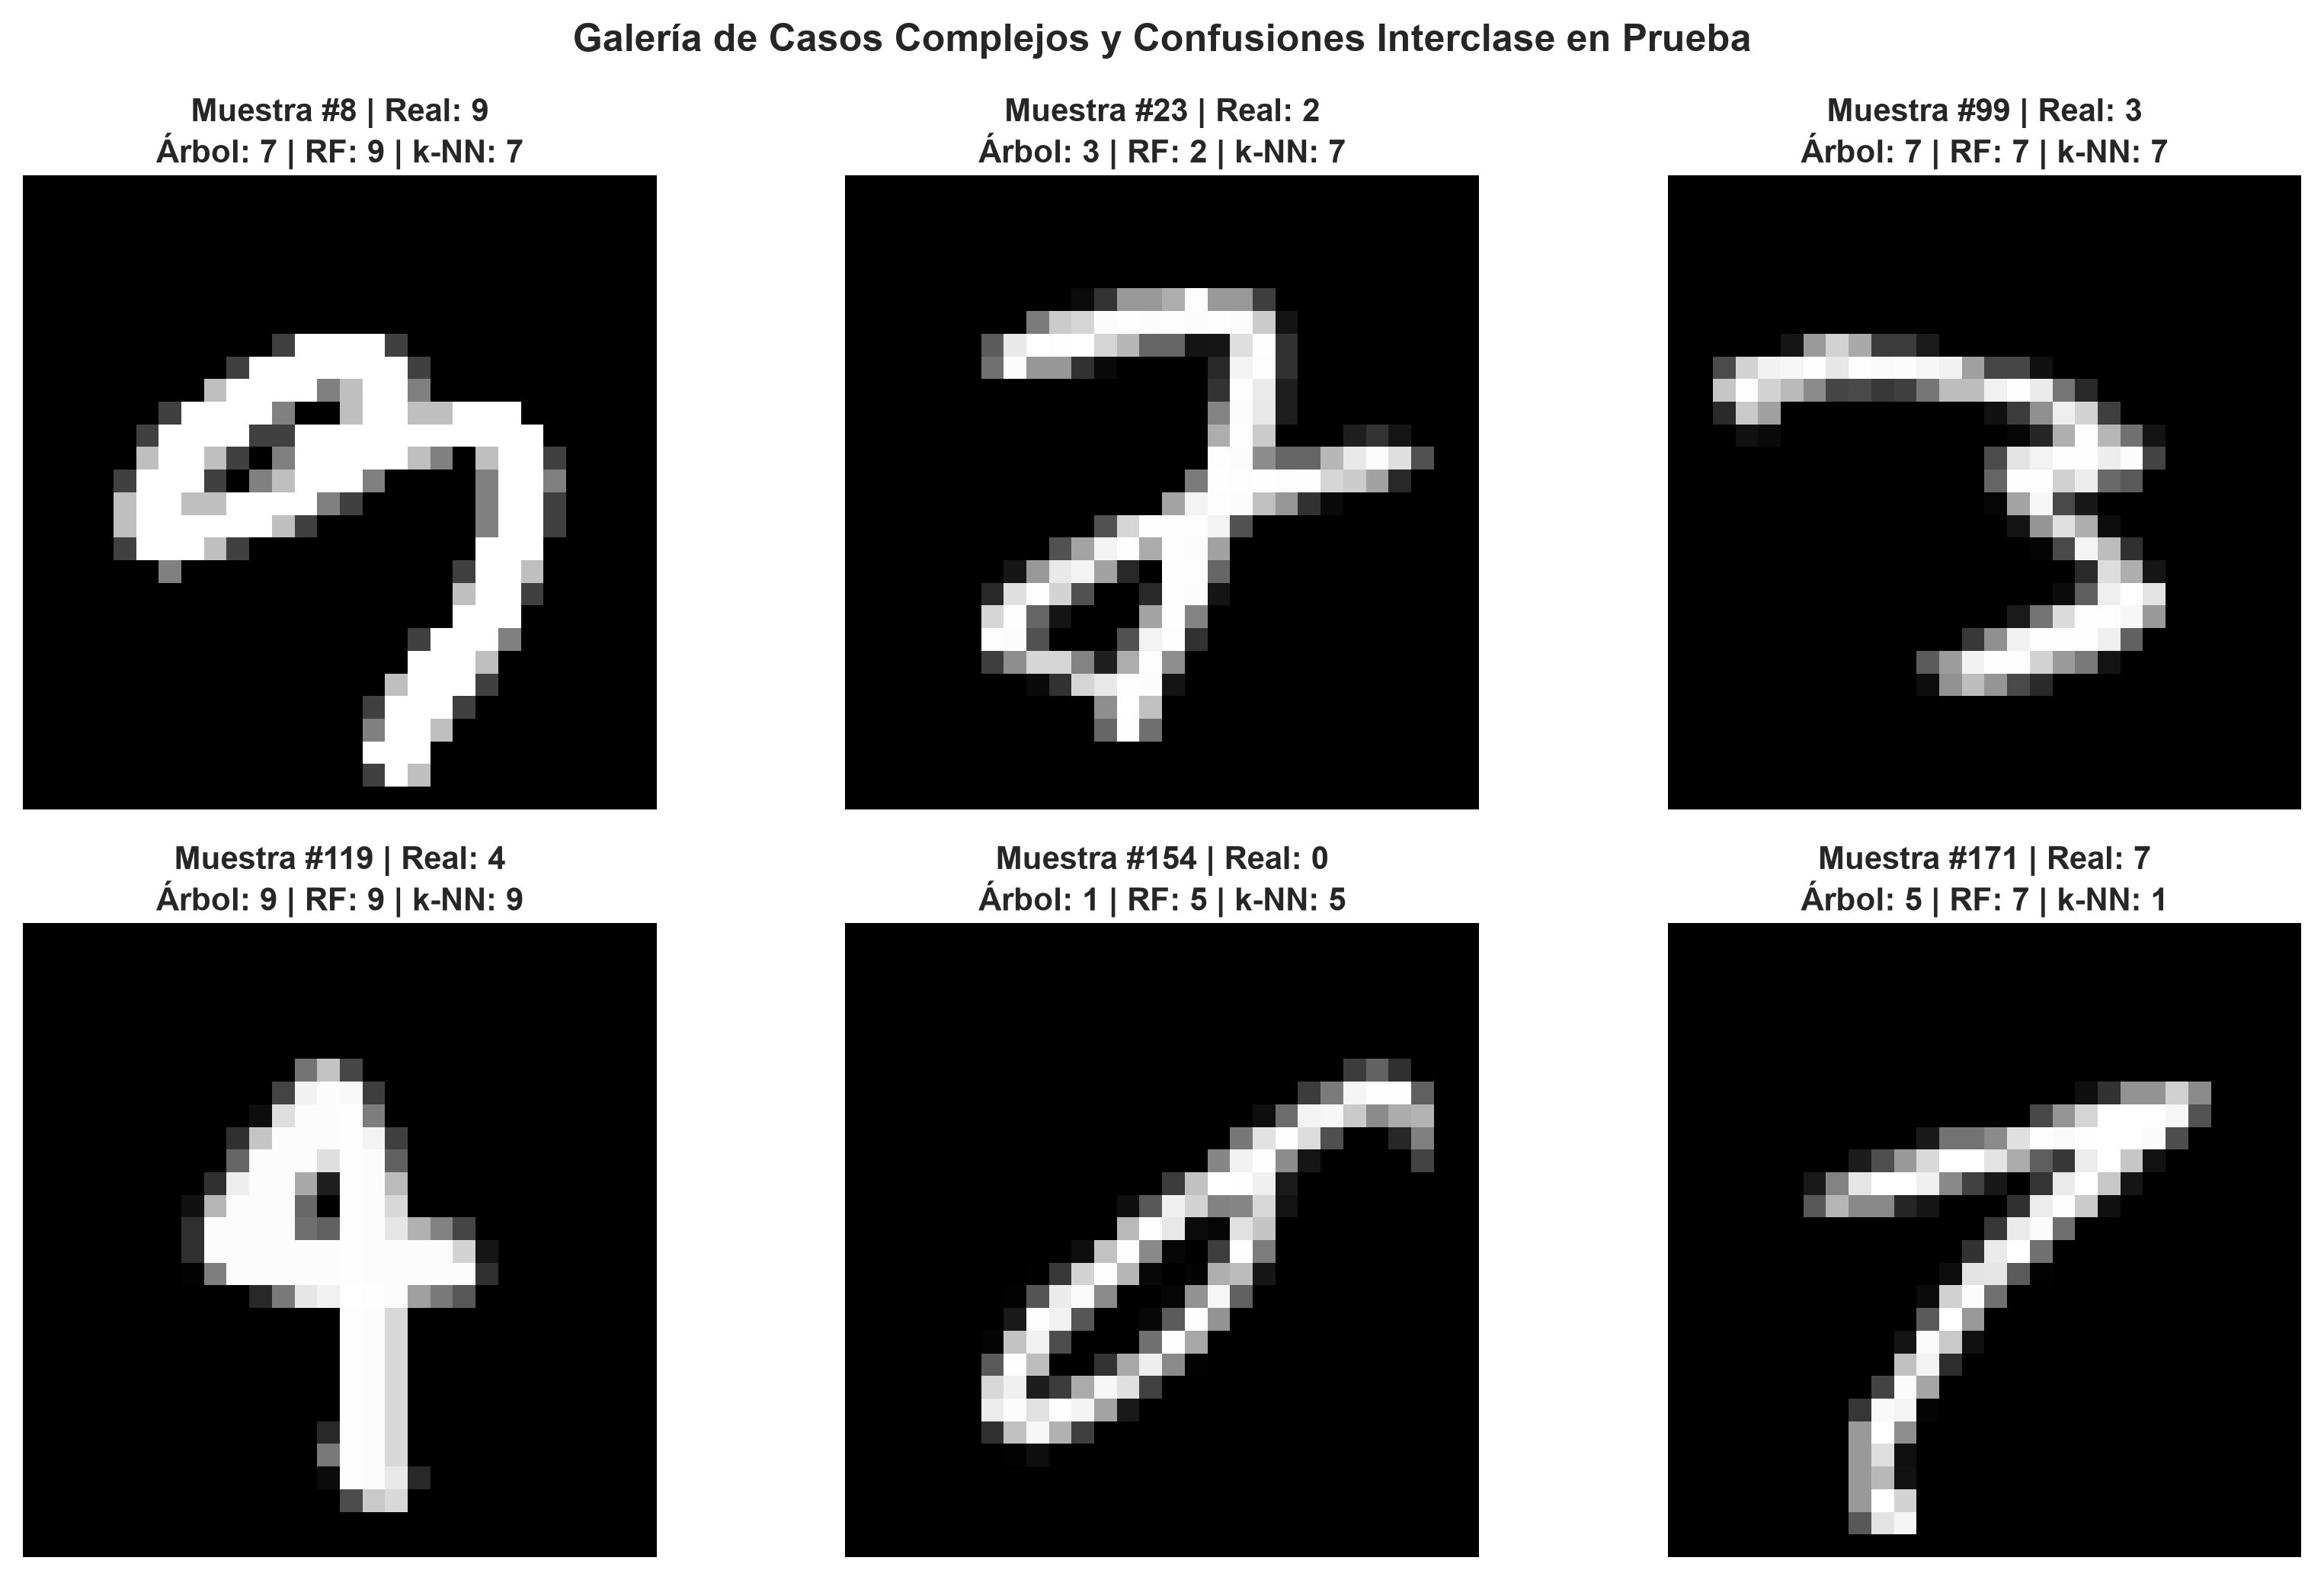
\includegraphics[width=0.85\textwidth]{images/ejemplos_mal_clasificados_grid.png}
    \caption{Galería de casos complejos y discrepancias interclase en el conjunto de prueba.}
    \label{fig:galeria_errores}
\end{figure}

\subsubsection*{2.7.6 Respuestas a las preguntas de comparación}
\begin{enumerate}[leftmargin=*]
    \item \textbf{¿Qué modelo obtuvo la mayor exactitud y el menor error en prueba? Cuantifiquen la diferencia respecto al segundo, o indiquen si hubo empate.}
    
    El modelo con mejor desempeño global en el conjunto de prueba fue \textbf{Random Forest}, alcanzando una exactitud de \textbf{94.80\,\%} y un error mínimo de \textbf{5.20\,\%}. Superó a su competidor más cercano, el clasificador \textbf{k-NN} (exactitud de \textbf{94.55\,\%} y error de \textbf{5.45\,\%}), por una diferencia positiva de \textbf{0.25 puntos porcentuales} (p. p.). Ambos clasificadores superaron categóricamente al Árbol de decisión simple (81.80\,\% de exactitud y 18.20\,\% de error), situándose Random Forest \textbf{13.00 p. p.} por encima de este último.
    
    \item \textbf{¿Qué modelo presentó la mayor brecha entre entrenamiento y prueba? Expliquen qué sugiere sin tomarla como prueba concluyente de sobreajuste. En k-NN, una observación de entrenamiento puede ser su propio vecino.}
    
    La mayor brecha de exactitud la presentó el \textbf{Árbol de decisión}, con una diferencia de \textbf{17.22 puntos porcentuales} (99.02\,\% en entrenamiento frente a 81.80\,\% en prueba). Esta notable brecha sugiere un claro sobreajuste (\textit{overfitting}), en el cual el árbol individual memorizó patrones de ruido y particularidades caligráficas locales del conjunto de entrenamiento al alcanzar una profundidad de 15 niveles sin podado.
    
    En contraste, k-NN exhibió la menor brecha aparente (\textbf{1.96 p. p.}, con 96.51\,\% en entrenamiento y 94.55\,\% en prueba). No obstante, esta métrica debe interpretarse con cautela: cuando se evalúa el conjunto de entrenamiento en k-NN, cada instancia evaluada es su propio vecino más cercano a distancia euclidiana cero, lo que infla de forma intrínseca la exactitud de entrenamiento sin que signifique una generalización paramétrica subyacente.
    
    \item \textbf{¿Qué confusión común o diferente observaron entre los modelos? Justifiquen qué clasificador recomendarían para esta tarea con al menos dos evidencias.}
    
    Se evidenciaron patrones de error característicos para cada modelo:
    \begin{itemize}[noitemsep]
        \item El Árbol de decisión concentra fallos severos en dígitos con contornos redondeados análogos (3 vs 5 con 14 casos, y 4 vs 9 con 11 casos).
        \item Random Forest distribuye los errores de manera más homogénea y en magnitudes mucho menores; su peor caso fue 7 confundido con 9 (7 casos).
        \item k-NN presentó confusiones asociadas a la dispersión de la distancia euclidiana en alta dimensión, confundiendo 2 con 7 (9 casos).
    \end{itemize}
    
    \textbf{Clasificador Recomendado:} Se recomienda de manera concluyente el modelo \textbf{Random Forest}, fundamentado en dos evidencias sólidas:
    \begin{itemize}[noitemsep]
        \item \textit{Evidencia 1 (Rendimiento predictivo superior):} Obtuvo la mayor exactitud en prueba (94.80\,\%) y el menor error (5.20\,\%), limitando la máxima confusión entre pares a tan solo 7 casos (frente a 14 del árbol y 9 de k-NN).
        \item \textit{Evidencia 2 (Eficiencia en inferencia):} Durante la predicción sobre las 2\,000 muestras de prueba, Random Forest tardó apenas \textbf{0.62 segundos} (0.31 ms por muestra), mientras que k-NN requirió \textbf{2.65 segundos} (más de 4 veces más lento) debido al costo de calcular distancias a 10\,000 vectores en 784 dimensiones. En un entorno productivo de digitalización masiva, Random Forest resulta mucho más escalable y rápido.
    \end{itemize}
\end{enumerate}

\subsection*{2.8 Habilidades blandas empleadas en la práctica}
A continuación se indican las habilidades blandas aplicadas y las acciones concretas realizadas:

\begin{itemize}[leftmargin=*,labelsep=0.3cm]
    \item[$\square$] \textbf{Liderazgo}
    \item[$\boxtimes$] \textbf{Trabajo en equipo}
    \item[$\boxtimes$] \textbf{Comunicación asertiva} 
    \item[$\square$] \textbf{La empatía}
    \item[$\boxtimes$] \textbf{Pensamiento crítico}
    \item[$\square$] \textbf{Flexibilidad}
    \item[$\square$] \textbf{La resolución de conflictos}
    \item[$\square$] \textbf{Adaptabilidad}
    \item[$\boxtimes$] \textbf{Responsabilidad} 
\end{itemize}

\subsection*{2.9 Conclusiones}
\begin{enumerate}[leftmargin=*]
    \item \textbf{Desempeño en prueba:} Random Forest demostró ser el clasificador más robusto y preciso, alcanzando una exactitud de 94.80\,\% y una tasa de error de solo 5.20\,\% en el conjunto de prueba de 2\,000 dígitos, superando a k-NN (94.55\,\%) y aventajando de manera contundente al Árbol de decisión simple (81.80\,\%) con una diferencia de 13.00 puntos porcentuales. Esto confirma experimentalmente la efectividad del aprendizaje por ensamble (\textit{bagging}) para mitigar la varianza individual y capturar las variaciones en los trazos manuscritos.
    
    \item \textbf{Diferencia entre entrenamiento y prueba:} El Árbol de decisión evidenció un severo sobreajuste (\textit{overfitting}) con una brecha de generalización de 17.22 puntos porcentuales (99.02\,\% en entrenamiento vs 81.80\,\% en prueba), derivado de ramificaciones excesivamente profundas en un espacio de 784 variables. En contraste, Random Forest redujo sustancialmente esta brecha a 5.13 p. p. gracias a la aleatorización de características. Por su parte, la brecha aparentemente baja de k-NN (1.96 p. p.) refleja la condición particular del método en la que los puntos de entrenamiento coinciden consigo mismos a distancia cero, lo que enfatiza la necesidad de evaluar el rendimiento real exclusivamente con datos de prueba no vistos.
\end{enumerate}

\subsection*{2.10 Recomendaciones}
Para ensayos futuros, se propone implementar una optimización sistemática de hiperparámetros mediante \textbf{validación cruzada estratificada de $k$ pliegues (\textit{Stratified $k$-Fold Cross Validation})} con $k = 5$, aplicada \textbf{exclusivamente sobre el conjunto de entrenamiento ($X_{\text{ent}}$)} mediante \texttt{GridSearchCV} o técnicas bayesianas.

De este modo, se podrán explorar y sintonizar parámetros clave (como \texttt{n\_estimators}, \texttt{max\_depth} y criterios de poda \texttt{ccp\_alpha} en Random Forest, así como diferentes métricas de distancia en k-NN) sin incurrir en fuga de información (\textit{data leakage}), manteniendo el conjunto de prueba de $2\,000$ observaciones completamente aislado hasta la evaluación final del modelo definitivo. Asimismo, se aconseja evaluar la aplicación de Análisis de Componentes Principales (PCA) como paso previo para reducir la dimensionalidad de 784 a unas 50 componentes, lo cual aceleraría drásticamente la velocidad de inferencia de k-NN sin comprometer sustancialmente la exactitud.

\subsection*{2.11 Referencias bibliográficas}
\begin{thebibliography}{9}
\bibitem{openml_mnist} Y. LeCun, C. Cortes y C. J. C. Burges, «mnist\_784», v. 1, OpenML, ID 554. [En línea]. Disponible: \url{https://www.openml.org/d/554}
\bibitem{sklearn_dt} Scikit-learn developers, «DecisionTreeClassifier», \textit{scikit-learn documentation}. [En línea]. Disponible: \url{https://scikit-learn.org/stable/modules/generated/sklearn.tree.DecisionTreeClassifier.html}
\bibitem{sklearn_rf} Scikit-learn developers, «RandomForestClassifier», \textit{scikit-learn documentation}. [En línea]. Disponible: \url{https://scikit-learn.org/stable/modules/generated/sklearn.ensemble.RandomForestClassifier.html}
\bibitem{sklearn_knn} Scikit-learn developers, «KNeighborsClassifier», \textit{scikit-learn documentation}. [En línea]. Disponible: \url{https://scikit-learn.org/stable/modules/generated/sklearn.neighbors.KNeighborsClassifier.html}
\bibitem{sklearn_accuracy} Scikit-learn developers, «accuracy\_score», \textit{scikit-learn documentation}. [En línea]. Disponible: \url{https://scikit-learn.org/stable/modules/generated/sklearn.metrics.accuracy_score.html}
\end{thebibliography}

\subsection*{2.12 Anexos}

\paragraph{Anexo A. Código de partida para preparar los datos}
A continuación se transcribe el bloque de partida provisto en la guía para la ingesta y partición del dataset:

\begin{lstlisting}
from sklearn.datasets import fetch_openml
from sklearn.model_selection import train_test_split

X, y = fetch_openml(data_id=554, as_frame=False, return_X_y=True)
X = X.astype("float32") / 255.0
y = y.astype("int64")

def tomar_muestra(X_base, y_base, n):
    X_muestra, _, y_muestra, _ = train_test_split(
        X_base, y_base, train_size=n, stratify=y_base,
        random_state=42
    )
    return X_muestra, y_muestra

X_ent, y_ent = tomar_muestra(X[:60000], y[:60000], 10000)
X_pru, y_pru = tomar_muestra(X[60000:], y[60000:], 2000)
print(X_ent.shape, X_pru.shape) # (10000, 784), (2000, 784)
\end{lstlisting}

\paragraph{Anexo B. Archivos para la entrega}
De acuerdo a lo estipulado en la guía, se generaron y entregan los siguientes artefactos:
\begin{itemize}[leftmargin=*]
    \item \textbf{Informe Técnico:} Documento formal en formato \LaTeX\ (\texttt{informe\_mnist.tex}) y su versión compilada en PDF (\texttt{informe\_mnist.pdf}), conteniendo la portada institucional de la UTA, la Tabla 2 con todas las métricas requeridas, las matrices de confusión analizadas, el ejemplo de error, la comparativa técnica fundamentada, habilidades blandas, conclusiones y recomendaciones.
    \item \textbf{Cuaderno interactivo de Jupyter (\texttt{.ipynb}):} Archivo \url{Taller_APE_MNIST_Arbol_RandomForest_kNN.ipynb} totalmente ejecutado, con todas las salidas, celdas de código reproducibles y visualizaciones embebidas desde la carga de MNIST hasta las matrices de confusión finales.
\end{itemize}

\end{document}
